\documentclass[12pt,a4paper,twoside,openright]{report}
\let\openright=\cleardoublepage



%%% Choose a language %%%

\newif\ifEN
% \ENtrue   % uncomment this for english
\ENfalse   % uncomment this for czech

%%% Configuration of the title page %%%

\def\ThesisTitleStyle{mff} % MFF style
%\def\ThesisTitleStyle{cuni} % uncomment for old-style with cuni.cz logo
%\def\ThesisTitleStyle{natur} % uncomment for nature faculty logo

\def\UKFaculty{Faculty of Mathematics and Physics}
%\def\UKFaculty{Faculty of Science}

\def\UKName{Charles University in Prague} % this is not used in the "mff" style

% Thesis type names, as used in several places in the title
\def\ThesisTypeTitle{\ifEN BACHELOR THESIS \else BAKALÁŘSKÁ PRÁCE \fi}
%\def\ThesisTypeTitle{\ifEN MASTER THESIS \else DIPLOMOVÁ PRÁCE \fi}
%\def\ThesisTypeTitle{\ifEN RIGOROUS THESIS \else RIGORÓZNÍ PRÁCE \fi}
%\def\ThesisTypeTitle{\ifEN DOCTORAL THESIS \else DISERTAČNÍ PRÁCE \fi}
\def\ThesisGenitive{\ifEN bachelor \else bakalářské \fi}
%\def\ThesisGenitive{\ifEN master \else diplomové \fi}
%\def\ThesisGenitive{\ifEN rigorous \else rigorózní \fi}
%\def\ThesisGenitive{\ifEN doctoral \else disertační \fi}
\def\ThesisAccusative{\ifEN bachelor \else bakalářskou \fi}
%\def\ThesisAccusative{\ifEN master \else diplomovou \fi}
%\def\ThesisAccusative{\ifEN rigorous \else rigorózní \fi}
%\def\ThesisAccusative{\ifEN doctoral \else disertační \fi}



%%% Fill in your details %%%

% (Note: \xxx is a "ToDo label" which makes the unfilled visible. Remove it.)
\def\ThesisTitle{Možnosti návrhového vzoru Entity-Component-System: případová studie}
\def\ThesisAuthor{Petr Kotáb}
\def\YearSubmitted{2024}

% department assigned to the thesis
\def\Department{Katedra softwaru a výuky informatiky}
% Is it a department (katedra), or an institute (ústav)?
\def\DeptType{Katedra}

\def\Supervisor{Mgr. Pavel Ježek, Ph.D.}
\def\SupervisorsDepartment{Katedra distribuovaných a spolehlivých systémů}

% Study programme and specialization
\def\StudyProgramme{Informatika }
\def\StudyBranch{Počítačová grafika, vidění a vývoj her}

\def\Dedication{%
Dedication. \xxx{It is nice to say thanks to supervisors, friends, family, book authors and food providers.}
}

\def\AbstractEN{%
\xxx{Abstracts are an abstract form of art. Use the most precise, shortest sentences that state what problem the thesis addresses, how it is approached, pinpoint the exact result achieved, and describe the applications and significance of the results. Highlight anything novel that was discovered or improved by the thesis. Maximum length is 200 words, but try to fit into 120. Abstracts are often used for deciding if a reviewer will be suitable for the thesis; a well-written abstract thus increases the probability of getting a reviewer who will like the thesis.}
% ABSTRACT IS NOT A COPY OF YOUR THESIS ASSIGNMENT!
}

\def\AbstractCS{%
\xxx{You will need to submit both Czech and English abstract to the SIS, no matter what language you use in the thesis. If writing in English, translate the contents of \texttt{\textbackslash{}AbstractEN} into this field. In case you do not speak czech, your supervisor should be able to help you with the translation.}
}

% 3 to 5 keywords (recommended), each enclosed in curly braces.
% Keywords are useful for indexing and searching for the theses by topic.
\def\Keywords{
    {návrhový vzor}
    {Entity-Component-System}
    {počítačové hry}
    {simulace}
    {případová studie}
}

% If your abstracts are long and do not fit in the infopage, you can make the
% fonts a bit smaller by this setting. (Also, you should try to compress your abstract more.)
% Alternatively, consider increasing the size of the page by uncommenting the
% geometry modification in thesis.tex.
\def\InfoPageFont{}
%\def\InfoPageFont{\small}  %uncomment to decrease font size

\ifEN\relax\else
% If you are writing a czech thesis, you additionally need to fill in the
% english translation of the metadata here!
\def\ThesisTitleEN{Exploring Options of Entity-Component-System Design Pattern: A Case Study}
\def\DepartmentEN{Department of software and computer science education}
\def\DeptTypeEN{Department}
\def\SupervisorsDepartmentEN{Department of Distributed and Dependable Systems}
\def\StudyProgrammeEN{Computer Science}
\def\StudyBranchEN{Computer Graphics, Vision and Game Development}
\def\KeywordsEN{
    {design pattern}
    {Entity-Component-System}
    {computer games}
    {simulation}
    {case study}
}
\fi


\usepackage[a-2u]{pdfx}

\ifEN\else\usepackage[czech,shorthands=off]{babel}\fi

% See https://en.wikipedia.org/wiki/Canons_of_page_construction before
% modifying the size of printable area. LaTeX defaults are great.
% If you feel it would help anything, you can enlarge the printable area a bit:
%\usepackage[textwidth=390pt,textheight=630pt]{geometry}
% The official recommendation expands the area quite a bit (looks pretty harsh):
%\usepackage[textwidth=145mm,textheight=247mm]{geometry}

%%% TYPICAL FONT CHOICES (uncomment what you like) %%%
% Recommended combo: Libertinus (autoselects Biolinum for sans) and everything
% else (math+tt) comes from Latin Modern)
\usepackage{lmodern}
\usepackage[mono=false]{libertinus}

% For the "classic" LaTeX fonts (very good for pure math theses), simply
% comment out the libertinus package above.

% IBM Plex font suite: nice, but requires us to fine-tune the sizes and does
% not directly support small caps (\textsc):
%\usepackage[usefilenames,RM={Scale=0.88},SS={Scale=0.88},SScon={Scale=0.88},TT={Scale=0.88},DefaultFeatures={Ligatures=Common}]{plex-otf}

% TeX Gyre combo (Pagella+Heros+Cursor)
%\usepackage{fontspec}
%\setmainfont{TeX Gyre Pagella}
%\setsansfont{TeX Gyre Heros}
%\setmonofont{TeX Gyre Cursor}

% some useful packages
\usepackage{microtype}
\usepackage{amsmath,amsfonts,amsthm,bm}
\usepackage{graphicx}
\usepackage{xcolor}
\usepackage{booktabs}
\usepackage{caption}
\usepackage{floatrow}
% \usepackage[htt]{hyphenat}
% \usepackage{afterpage}

% Bibliography formatting.
% CHECK THE REQUIREMENTS OF YOUR DEPARTMENT AND FACULTY ON THE CITATION FORMAT!
%
% These are relatively "safe" default options that most people use:
\usepackage[natbib,style=numeric,sorting=none]{biblatex}
% alternative with alphanumeric citations (more informative than numbers, and
% more common in computer science journals):
%\usepackage[natbib,style=alphabetic]{biblatex}
%
% ALTERNATIVES THAT CONFORM TO ISO690
% ISO690 is not the greatest citation format ever, but may be formally
% required at Charles University, depending on your faculty and department.
%\usepackage[natbib,style=iso-numeric,sorting=none]{biblatex}
%\usepackage[natbib,style=iso-alphabetic]{biblatex}
% You might want to add extra options such as `maxbibnames=6,maxcitenames=2`
% here to further conform to some of the formatting requirements (see below for
% details). Again, consult your faculty rules.
%
% Additional option choices:
%  - add `giveninits=true` to typeset "E. A. Poe" instead of full Edgar Allan
%  - `terseinits=true` additionally shortens it to nature-like "Poe EA"
%  - add `maxnames=10` to limit (or loosen) the maximum number of authors in
%    bibliography entry before shortening to `et al.` (useful when referring to
%    book collections that may have hundreds of authors)
%  - use `maxcitenames=2` to finetune the amount of authors listed in text-cite
%    commands (\citet). Corresponding option that only affects the bibliography
%    is `maxbibnames=10`.
%  - `sorting=none` causes the bibliography list to be ordered by the order of
%    citation as they appear in the text, which is usually the desired behavior
%    with numeric citations. Additionally you can use a style like
%    `numeric-comp` that compresses the long lists of citations such as
%    [1,2,3,4,5,6,7,8] to simpler [1--8]. This is especially useful if you plan
%    to add tremendous amounts of citations, as usual in life sciences and
%    bioinformatics.
%  - if you don't like the "In:" appearing in the bibliography, use the
%    extended style (`ext-numeric` or `ext-alphabetic`), and add option
%    `articlein=false`.
%
% possibly reverse the names of the authors with the default styles:
%\DeclareNameAlias{default}{family-given}

% load the file with bibliography entries
\addbibresource{refs.bib}

% remove this if you won't use fancy verbatim environments
\usepackage{fancyvrb}

% remove this if you won't typeset TikZ graphics
\usepackage{tikz}
\usetikzlibrary{positioning} %add libraries as needed (shapes, decorations, ...)

% remove this if you won't typeset any pseudocode
\usepackage{algpseudocode}
\usepackage{algorithm}

% remove this if you won't list any source code
\usepackage{listings}


\hypersetup{unicode}
\hypersetup{breaklinks=true}

\usepackage[noabbrev]{cleveref}

% 
% various forms of TODOs (you should remove this before submitting)
\usepackage[textsize=tiny, backgroundcolor=yellow!25, linecolor=black!25]{todonotes}
\newcommand{\xxx}[1]{\textcolor{red!}{#1}}

 % remove this before compiling the final version


% use this for typesetting a chapter without a number, e.g. intro and outro
\def\chapwithtoc#1{\chapter*{#1}\addcontentsline{toc}{chapter}{#1}}

% If there is a line/figure overflowing into page margin, this will make the
% problem evident by drawing a thick black line at the overflowing spot. You
% should not disable this.
\overfullrule=3mm

% The maximum stretching of a space. Increasing this makes the text a bit more
% sloppy, but may prevent the overflows by moving words to next line.
\emergencystretch=1em

\ifEN
\theoremstyle{plain}
\newtheorem{thm}{Theorem}
\newtheorem{lemma}[thm]{Lemma}
\newtheorem{claim}[thm]{Claim}
\newtheorem{defn}{Definition}
\theoremstyle{remark}
\newtheorem*{cor}{Corollary}
\else
\theoremstyle{plain}
\newtheorem{thm}{Věta}
\newtheorem{lemma}{Lemma}
\newtheorem{claim}{Tvrzení}
\newtheorem{defn}{Definice}
\theoremstyle{remark}
\newtheorem*{cor}{Důsledek}
\fi

\newenvironment{myproof}{
  \par\medskip\noindent
  \textit{\ifEN Proof \else Důkaz \fi}.
}{
\newline
\rightline{$\qedsymbol$}
}

% real/natural numbers
\newcommand{\R}{\mathbb{R}}
\newcommand{\N}{\mathbb{N}}

% asymptotic complexity
\newcommand{\asy}[1]{\mathcal{O}(#1)}

% listings and default lstlisting config (remove if unused)
\DeclareNewFloatType{listing}{}
\floatsetup[listing]{style=ruled}

\DeclareCaptionStyle{thesis}{style=base,font={small,sf},labelfont=bf,labelsep=quad}
\captionsetup{style=thesis}
\captionsetup[algorithm]{style=thesis,singlelinecheck=off}
\captionsetup[listing]{style=thesis,singlelinecheck=off}

% Customization of algorithmic environment (comment style)
\renewcommand{\algorithmiccomment}[1]{\textcolor{black!25}{\dotfill\sffamily\itshape#1}}

% Uncomment for table captions on top. This is sometimes recommended by the
% style guide, and even required for some publication types.
%\floatsetup[table]{capposition=top}
%
% (Opinionated rant:) Captions on top are not "compatible" with the general
% guideline that the tables should be formatted to be quickly visually
% comprehensible and *beautiful* in general (like figures), and that the table
% "head" row (with column names) should alone communicate most of the content
% and interpretation of the table. If you just need to show a long boring list
% of numbers (because you have to), either put some effort into showing the
% data in an attractive figure-table, or move the data to an attachment and
% refer to it, so that the boredom does not impact the main text flow.
%
% You can make the top-captions look much less ugly by aligning the widths of
% the caption and the table, with setting `framefit=yes`, as shown below.  This
% additionally requires some extra markup in your {table} environments; see the
% comments in the example table in `ch2.tex` for details.
%\floatsetup[table]{capposition=top,framefit=yes}

\ifEN\floatname{listing}{Listing}
\else\floatname{listing}{Výpis kódu}\fi
\lstset{ % use this to define styling for any other language
  language=C++,
  tabsize=2,
  showstringspaces=false,
  basicstyle=\footnotesize\tt\color{black!75},
  identifierstyle=\bfseries\color{black},
  commentstyle=\color{green!50!black},
  stringstyle=\color{red!50!black},
  keywordstyle=\color{blue!75!black}}

% Czech versions of the used cleveref references (It's not as convenient as in
% English because of declension, cleveref is limited to sg/pl nominative. Use
% plain \ref to dodge that.)
\ifEN\relax\else
\crefname{chapter}{kapitola}{kapitoly}
\Crefname{chapter}{Kapitola}{Kapitoly}
\crefname{section}{sekce}{sekce}
\Crefname{section}{Sekce}{Sekce}
\crefname{subsection}{sekce}{sekce}
\Crefname{subsection}{Sekce}{Sekce}
\crefname{subsubsection}{sekce}{sekce}
\Crefname{subsubsection}{Sekce}{Sekce}
\crefname{figure}{obrázek}{obrázky}
\Crefname{figure}{Obrázek}{Obrázky}
\crefname{table}{tabulka}{tabulky}
\Crefname{table}{Tabulka}{Tabulky}
\crefname{listing}{výpis}{výpisy}
\Crefname{listing}{Výpis}{Výpisy}
\floatname{algorithm}{Algoritmus}
\crefname{algorithm}{algoritmus}{algoritmy}
\Crefname{algorithm}{Algoritmus}{Algoritmy}
\newcommand{\crefpairconjunction}{ a~}
\newcommand{\crefrangeconjunction}{ a~}
\fi
 % use this file for various custom definitions

\begin{document}

% the layout is mandatory, edit only in dire circumstances

\pagestyle{empty}
\hypersetup{pageanchor=false}
\begin{center}

% top part of the layout, this actually differs between faculties

\def\ThesisTitleXmff{%
  \ifEN
    \centerline{\mbox{
\includegraphics[width=166mm]{img/logo-en.pdf}}}
  \else
    \centerline{\mbox{
\includegraphics[width=166mm]{img/logo-cs.pdf}}}
  \fi
  \vspace{-8mm}\vfill%
  {\bf\Large\ThesisTypeTitle}
  \vfill%
  {\LARGE\ThesisAuthor}\par
  \vspace{15mm}%
  {\LARGE\bfseries\ThesisTitle}
  \vfill%
  \Department}
\def\ThesisTitleCuniLogo#1{%
  {\large\UKName\par\medskip\par\UKFaculty }
  \vfill%
  {\bf\Large\ThesisTypeTitle}
  \vfill%
  \includegraphics[width=70mm]{#1}
  \vfill%
  {\LARGE\ThesisAuthor}\par
  \vspace{15mm}%
  {\LARGE\bfseries\ThesisTitle}
  \vfill%
  \Department\par}
\def\ThesisTitleXcuni{\ThesisTitleCuniLogo{img/uklogo.pdf}}
\def\ThesisTitleXnatur{\ThesisTitleCuniLogo{img/naturlogo.pdf}}

% choose the correct page and print it
\csname ThesisTitleX\ThesisTitleStyle\endcsname
% latex corner: X is the new @

\vfill

{
\centerline{\vbox{\halign{\hbox to 0.45\hsize{\hfil #}&\hskip 0.5em\parbox[t]{0.45\hsize}{\raggedright #}\cr
\ifEN Supervisor of the \ThesisGenitive thesis:
\else Vedoucí \ThesisGenitive práce: \fi
& \Supervisor \cr
\noalign{\vspace{2mm}}
\ifEN Study programme: \else Studijní program: \fi
& \StudyProgramme \cr
\noalign{\vspace{2mm}}
\ifEN Study branch: \else Studijní obor: \fi
& \StudyBranch \cr
}}}}

\vfill

\ifEN Prague \else Praha \fi
\YearSubmitted

\end{center}

\newpage

% remember to sign this!
\openright
\hypersetup{pageanchor=true}
\pagestyle{plain}
\pagenumbering{roman}
\vglue 0pt plus 1fill

\ifEN
\noindent
I declare that I carried out this \ThesisAccusative thesis independently, and only with the cited
sources, literature and other professional sources. It has not been used to obtain another
or the same degree.
\else
\noindent
Prohlašuji, že jsem tuto \ThesisAccusative práci vypracoval(a) samostatně a výhradně
s~použitím citovaných pramenů, literatury a dalších odborných zdrojů.
Tato práce nebyla využita k získání jiného nebo stejného titulu.
\fi

\ifEN
\medskip\noindent
I understand that my work relates to the rights and obligations under the Act No.~121/2000 Sb.,
the Copyright Act, as amended, in particular the fact that the Charles
University has the right to conclude a license agreement on the use of this
work as a school work pursuant to Section 60 subsection 1 of the Copyright~Act.
\else
\medskip\noindent
Beru na~vědomí, že se na moji práci vztahují práva a povinnosti vyplývající
ze zákona č. 121/2000 Sb., autorského zákona v~platném znění, zejména skutečnost,
že Univerzita Karlova má právo na~uzavření licenční smlouvy o~užití této
práce jako školního díla podle §60 odst. 1 autorského zákona.
\fi

\vspace{10mm}


\ifEN
\hbox{\hbox to 0.5\hsize{%
In \hbox to 6em{\dotfill} date \hbox to 6em{\dotfill}
\hss}\hbox to 0.5\hsize{\dotfill\quad}}
\smallskip
\hbox{\hbox to 0.5\hsize{}\hbox to 0.5\hsize{\hfil Author's signature\hfil}}
\else
\hbox{\hbox to 0.5\hsize{%
V \hbox to 6em{\dotfill} dne \hbox to 6em{\dotfill}
\hss}\hbox to 0.5\hsize{\dotfill\quad}}
\smallskip
\hbox{\hbox to 0.5\hsize{}\hbox to 0.5\hsize{\hfil Podpis autora\hfil}}
\fi

\vspace{20mm}
\newpage

% dedication

\openright

\noindent
\Dedication

\newpage

% mandatory information page

\openright

\vbox to 0.49\vsize{\InfoPageFont
\setlength\parindent{0mm}
\setlength\parskip{5mm}

\ifEN Title: \else Název práce: \fi
\ThesisTitle

\ifEN Author: \else Autor: \fi
\ThesisAuthor

\DeptType:
\Department

\ifEN Supervisor: \else Vedoucí \ThesisGenitive práce: \fi
\Supervisor, \SupervisorsDepartment

\ifEN Abstract: \AbstractEN \else Abstrakt: \AbstractCS \fi

\ifEN Keywords: \else Klíčová slova: \fi
\Keywords

\vss}\ifEN\relax\else\nobreak\vbox to 0.49\vsize{\InfoPageFont
\setlength\parindent{0mm}
\setlength\parskip{5mm}

Title:
\ThesisTitleEN

Author:
\ThesisAuthor

\DeptTypeEN:
\DepartmentEN

Supervisor:
\Supervisor, \SupervisorsDepartmentEN

Abstract:
\AbstractEN

Keywords:
\KeywordsEN

\vss}
\fi

\newpage

\openright
\pagestyle{plain}
\pagenumbering{arabic}
\setcounter{page}{1}


\tableofcontents

\chapter{Úvod}

Vytváření her je komplexní proces, který zahrnuje mnoho fází, včetně prototypování a iterací. Často se ocitneme v situaci, kdy je nezbytné výrazně upravit již existující kód. Z tohoto důvodu je klíčová vysoká flexibilita architektury kódu.

Jedním z přístupů k řešení tohoto problému je využití návrhového vzoru Component, který poskytuje vysokou míru flexibility. Tento návrhový vzor je běžně používán v herních frameworcích a enginech, jako je například Unity (koncept MonoBehaviour) nebo MonoGame (koncept GameComponent). Návrhový vzor Component je dobře představen v knize Game Programming Patterns~\cite{nystrom2014game}.

Nicméně existují pokročilejší přístupy, které mohou nabídnout ještě lepší flexibilitu a výkon. Jedním takovím je návrhový vzor Entity-Component-System (ECS).  I přesto, že se v současné době nepoužíva tak často jako návrhový vzor Component, tak nabízí značné výhody při tvorbě her. Proto se na něj v této práci zaměříme. Tento návrhový vzor je dobře rozebrán v sérii článků s názvem ECS back and forth~\cite{Caini_2019}.

\section{Entity-Component-System}
ECS je návrhový vzor používaný pro vývoj her. Jeho základními stavebními kameny jsou entity, komponenty a systémy.

\begin{enumerate}
    \item \textbf{Entita (Entity):} Reprezentuje objekt v herní scéně, může být cokoliv od hráče po strom nebo zvíře.
    \item \textbf{Komponenta (Component):} Entita je složena z komponent, které ji popisují. Komponenty obsahují pouze data a žádnou herní logiku. Například hráč může mít komponentu Control, která popisuje, jak se ovládá, strom může mít komponentu Resource, která popisuje, kolik dřeva hráč získá, pokud jej pokácí, a zvíře může mít komponentu PathFollow, která popisuje cestu, po které se pohybuje. Všechny tři entity mohou mít komponenty Appearance, která popisuje, jak daný objekt vypadá, a Position, popisující, kde se daný objekt nachází v herní scéně. Dále hráč a zvíře mohou mít komponentu Movement, popisující jejich pohyb.
    \item \textbf{Systém (System):} Obsahuje herní logiku. Systémy pracují nad určitou množinou komponent. V každé iteraci vezmou všechny entity obsahující tuto množinu komponent a provedou nad nimi určité operace. Například:
    \begin{itemize}
        \item \textbf{InputSystem:} Pracuje nad entitami s komponentami Control a Position, řídí logiku jejich ovládání.
        \item \textbf{PathMovementSystem:} Pracuje nad entitami s komponentami PathFollow a Movement, řídí logiku jejich pohybu po cestě.
        \item \textbf{RenderSystem:} Pracuje nad entitami s komponentou Appearance a řídí logiku jejich vykreslení.
    \end{itemize}
\end{enumerate}

ECS nejenže poskytuje vysokou flexibilitu, ale také vyniká v oblasti výkonu. Jeho flexibilitu a výkon si více rozebereme v~\cref{chap:ecs} \xxx{poresit sklonovani u linku}. Mezi cíle této práce bude patřit prozkoumat možnosti, které tento návrhový vzor přináší, a ukázat výhody, které nám ECS může poskytnout v porovnání s návrhovým vzorem Component.

\section{ECS knihovny}
Aby bylo možné efektivně využívat návrhový vzor ECS, je nezbytné implementovat odpovídající infrastrukturu. Samotná implementace této infrastruktury představuje obtížnou a časově náročnou úlohu, což vede mnoho vývojářů k volbě již existujících knihoven implementujících infrastrukturu pro tento návrhový vzor.

V této práci se zaměříme na knihovny pro programovací jazyk C\#, neboť se jedná o programovací jazyk běžně používaný pro hry a aplikace. I když se omezíme pouze na C\#, existuje velké množství těchto knihoven.

Jedním ze způsobů jak si vývojáři mohou vybrat ECS knihovnu je použít porovnání. CSharpECSComparison~\cite{CSharpECSComparison} je projekt na platformě GitHub, který porovnává populární ECS knihovny pro C\# na základě funkcionalit, vlastností a závislostí. Vývojář by si tedy mohl říci, které vlastnosti a funkcionality by od takové knihovny požadoval a na základě toho si vybrat. Ovšem možnosti co nám jednotlivé ECS knihovny nabízejí se tolik neliší, proto dává smysl porovnávat jednotlivé knihovny na základě výkonu. Bohužel CSharpECSComparison nám neposkytuje žádné informace o výkonu jednotlivých knihoven.

Ecs.CSharp.Benchmark~\cite{EcsCsharpBenchmark} je projekt na platforme GitHub, který provádí jednoduché výkonnostní testy ECS knihoven pro C\#. Výsledky těchto testů mohou být užitečné při výběru knihovny na základě výkonu. Problém však může spočívat v tom, že tyto testy jsou příliš jednoduché. Každý test, který Ecs.CSharp.Benchmark provádí, pracuje pouze s velmi jednoduchými komponentami, kde každá komponenta obsahuje pouze jedno celé číslo. Testy jsou rozděleny do několika sad. První sada vytváří entity s těmito komponentami. Druhá sada spouští jednoduché systémy, které pouze sčítají výše zmíněná celá čísla na těchto komponentách.

Jelikož jsou testy příliš jednoduché, v případě rozsáhlejšího projektu, jako je hra, by se výsledky mohly lišit. Jednotlivé entity mohou mít velké množství komponent, z nichž každá může být složitější. Systémy mohou být také mnohem komplexnější a provádět mnohem složitější úkoly než pouhé sčítání celých čísel.

Jedním ze způsobů, jak by bylo možné lépe porovnat výkon jednotlivých ECS knihoven, by bylo vytvoření hry, na které by bylo možné měřit výkon jednotlivých knihoven. Taková hra by musela být nezávislá na konkrétní ECS knihovně. Měla by také obsahovat netriviálně velký svět s větším počtem entit. To by nám umožnilo lépe provádět měření. Jedním z cílů této práce bude vytvoření takovéto hry.

Poté, co budeme mít tuto hru k dispozici, bude možné vytvořit výkonnostní test, který by dokázal změřit výkon příslušné ECS knihovny na této hře. Pomocí tohoto testu bude možné udělat výkonostní porovnání jednotlivých ECS knihoven. Vytvoření tohoto porovnání bude dalším cílem této práce.

Zároveň takto vytvořená hra pro nás bude velice užitečná neboť nám pomůže při průzkumu možností návrhové vzoru ECS, což je jedním z cílů této práce.

\section{Abstrakční vrstva}
Vzhledem k tomu, že plánovanou hru budeme chtít využít k porovnávání různých ECS knihoven, je nezbytné navrhnout ji tak, aby fungovala nezávisle na konkrétní ECS knihovně. S ohledem na odlišné API jednotlivých ECS knihoven je nezbytné vytvořit abstrakční vrstvu pro ECS. Pro každou knihovnu, kterou budeme chtít porovnávat, poskytneme implementaci této vrstvy. Samotná hra poté pracuje s touto abstrakční vrstvou.

Vytvoření takovéto vrstvy představuje netriviální úkol, navzdory podobnosti rozhraní jednotlivých ECS knihoven. Významný rozdíl spočívá v rozhraní systémů, které se výrazně liší mezi jednotlivými knihovnami.

\section{Cíle práce}
Pro shrnutí, tato práce bude mít následující cíle:
\begin{enumerate}
    \item[h1)] Vytvořit hru pomocí ECS, která bude nezávislá na konkrétní ECS knihovně.
    \item[h2)] Pomocí vytvořené hry porovnat relativní výkon populárních ECS knihoven pro programovací jazyk C\#.
\end{enumerate}
S využitím této hry také budeme chtít:
\begin{enumerate}
    \item[v1)] Prozkoumat možnosti návrhového vzoru ECS.
    \item[v2)] Ukázat výhody, které nám ECS může nabídnout oproti návrhovému vzoru Component.
\end{enumerate}














\iffalse
\chapwithtoc{Introduction}

Introduction should answer the following questions, ideally in this order:
\begin{enumerate}
\item What is the nature of the problem the thesis is addressing?
\item What is the common approach for solving that problem now?
\item How this thesis approaches the problem?
\item What are the results? Did something improve?
\item What can the reader expect in the individual chapters of the thesis?
\end{enumerate}

Expected length of the introduction is between 1--4 pages. Longer introductions may require sub-sectioning with appropriate headings --- use \texttt{\textbackslash{}section*} to avoid numbering (with section names like `Motivation' and `Related work'), but try to avoid lengthy discussion of anything specific. Any ``real science'' (definitions, theorems, methods, data) should go into other chapters.
\todo{You may notice that this paragraph briefly shows different ``types'' of `quotes' in TeX, and the usage difference between a hyphen (-), en-dash (--) and em-dash (---).}

It is very advisable to skim through a book about scientific English writing before starting the thesis. I can recommend `\citetitle{glasman2010science}' by \citet{glasman2010science}.
\fi
\chapter{Hra}
V této kapitole si specifikujeme jak bude vypadat naše hra. Prvně si rozebereme jaké vlastnosti od ní vyžadujeme a následně provedeme samotnou specifikaci.

\section{Herní požadavky}
Nyní si upřesníme požadavky co chceme od naší hry, následně také zvolíme herní žánr.

Než budeme pokračovat, připomeňme si prvně, že naší hru chceme použít pro měření výkonu ECS knihoven. Budeme tedy chtít aby byla nezávislá na konkrétní ECS knihovně. Konkrétní ECS knihovnu bude možné zvolit před spuštěním hry.

\subsection{Charakteristiky hry}
\label{sec:game-characteristics}
Aby nám naše hra napomohla ke splnění práce, budeme chtít aby splňovala následující charakteristiky:

\begin{enumerate}
    \item \textbf{Nezávislost na konkrétní ECS knihovně:} Nezávislost na konkrétní ECS knihovně pro nás bude důležitá, abychom hru mohli použít pro měření výkonu jednotlivých knihoven. Hra bude namísto konkrétní ECS knihovny pracovat pouze s abstrakční vrstvou. Bude pro nás žádoucí aby se výkon naší hry bežící s konkretní ECS knihovnou, implementující abstrakční vrstvu, blížil k výkonu hry, která by používala pouze konkrétní ECS knihovnu bez abstrakční vrstvy.

    \item \textbf{Hra by neměla využívat velmi častého přidávání a odebírání komponent:} Přidaní a odebraní komponenty představuje pro některé ECS knihovny náročnější operaci. Ovšem to jestli hra využívá velmi častého přidávání a odebírání komponent je závislé z velké části na implementaci. Kdyby naše hra používala velmi častého přidávání a odebírání komponent, došlo by k znevýhodnění některých ECS knihoven, které by jinak na tom mohli být výkonnostně lépe. Ovšem je nutné zmínit, že odebírání komponent v některých případech nelze předejít. Typickým příkladem bývá odebírání entity například v případě její smrti.
    
    Ukažme si na příkladu, proč je velmi časté přidávání a odebírání komponent závislé z velké části na implementaci. Konkrétně bychom chtěli reprezentovat efekt toho, že entita hladoví. Pokud by nám velmi časté přidávání a odebírání komponent nevadilo, tak by jeden z typických přístupů byl vytvořit \verb|Starvation| komponentu a přidat jí na každou entitu, která začne hladovět. V případě, že se příslušná entita nasytí jídlem, tak přestane hladovět a dojde k odebrání této komponenty. Pokud bychom chtěli stejnou mechaniku navrhnout bez častého přidávání a odebírání komponent, tak jeden z možných způsobů by byl dát každé entitě co může hladovět \texttt{Hunger} komponentu, ve které by byl flag \verb|Starvation| který by rozhodoval o tom jestli daná entita hladoví či nikoliv.
    
    \item \textbf{Velký počet entit:} Velký počet entit nám usnadní měření výkonu naší hry. Také nám zaručí, že systémy budou vykonávat netriviální množství práce. Zároveň si tím vyzkoušíme velký výkon, kterým ECS disponuje. Velký počet entit nám také implikuje větší herní svět.
    
    \item \textbf{Adekvátní složitost hry:} Bude pro nás důležité aby naše hra nebyla příliš jednoduchá. Budeme se chtít vyhnout tomu, aby naše měření nebylo jenom dalším jednoduchým měřením výkonu. Ovšem taky si musíme dát pozor na to aby nebyla příliš složitá, jelikož to by odvádělo pozornost od problému, který řešíme.
\end{enumerate}


% \\
% \xxx{Jaka charakteristiky by nase hra mela mit?}
% \\
% \xxx{- Velky pocet entit.}
% \\
% \xxx{- Hra musi byt dostatecne slozita aby vysledek mel prakticky smysl.}
% \\
% \xxx{- Hra nesmi byt prislis slozita aby slozitost neodvadela od problemu.}
% \\
% \xxx{- Hra by nemela vyuzivat casteho pridavani/odebirani komponent.}
% \\
% \xxx{-- Kdyby ano, nektere knihovny by byli zvyhodnene.}

\subsection{Simulace}
Žánrem naší hry bude simulace, ale řekněme si nejprve co to vlastně je. Simulace je žánr video her, který se snaží simulovat agenty v jejich prostředí. U nás agenti budou vesničané a jejich prostředí bude příroda.

Proč jsme zvolili právě simulaci? Pro simulaci je jednodušší (oproti ostatním žánrům) vymyslet herní design, který má velký počet entit a netriviálně velký svět. Další velkou výhodou je malí vliv uživatele na průběh hry, to nám umožní lépe provádět měření. Konkrétně v naší hře bude hráč spíše pozorovatel, který sleduje jak simulace probíhá.

% \\
% \xxx{Proc jsme zvolili simulaci?}
% \\
% \xxx{- Velky pocet entit.}
% \\
% \xxx{- Mali vliv uzivatele na prubeh hry.}

\section{Herní specifikace}
\label{sec:game-spec}
% intro
Nyní si představíme specifikaci naší hry. Celá hra se dá rozdělit na dva hlavní prvky. Konkrétně svět a vesnice. Specifikujeme si tedy každý z nich.

Prvně než si začneme specifikovat jednotlivé prvky, je nutné upřesnit, že se jedná o 2D hru. Hráč v této hře zastává roli pozorovatele a celí svět pozoruje skrze kameru pohledem ze shora. Ovládá pouze pozici a přiblížení této kamery.

% svet
% - nahodne generovany
% - biomes
% - resources
% - - trees
% - - rocks
% - - iron
\subsection{Herní svět}
\label{sec:game-world}
Herní svět je náhodně generovaný s pevnou velikostí a skládá se z několika biomů. Každý biom je reprezentován jinou barvou a nacházejí se v něm odlišné suroviny. Zároveň pro každý biom je určeno zda po něm mohou vesničané chodit nebo stavět. Herní svět obsahuje následující biomy:

\begin{enumerate}
    \item \textit{Voda} (\verb|Water|): Reprezentuje vodní plochu. Není na ní možné chodit ani stavět.
    \item \textit{Pláž} (\verb|Beach|): Jedná se o písečné oblasti v okolí \textit{vody}. Je na ní možné chodit i stavět.
    \item \textit{Louka} (\verb|Plain|): Na \textit{louce} je možné chodit i stavět. Je na ni možné najít \textit{jeleny}.
    \item \textit{Les} (\verb|Forest|): V \textit{lese} je možné chodit i stavět. Nachází se v něm velké množství \textit{stromů}.
    \item \textit{Hora} (\verb|Mountain|): Jedná se o kamenitou \textit{horu}. Je možné na ní chodit i stavět. Nachází se na ní \textit{naleziště kamene}.
    \item \textit{Vysoká hora} (\verb|High Mountain|): \textit{Vysoká hora} je vždy obklopena \textit{horou}. Je pokryta sněhovou plochou. Je možné na ní chodit ale není možné na ní stavět. Nachází se na ní \textit{naleziště železné rudy}.
\end{enumerate}

Jak již bylo zmíněno v jednotlivých biomech se mohou nacházet suroviny. Suroviny se rozdělují do několika typů. Typ suroviny udává jak dlouho trvá ji sklidit, jaký předmět lze získat po jejím sklizení a počet těchto předmětů, který lze získat po jejím sklizení. Hra obsahuje následující suroviny:

\begin{enumerate}
    \item \textit{Strom} (\verb|Tree|): Po pokácení \textit{stromu} lze získat předmět \textit{dřeva}. \textit{Stromy} se nacházejí ve velkém množství v biomu \textit{lesa}.
    \item \textit{Naleziště kamene} (\verb|Rock|): Sklizením \textit{naleziště kamene} je možné získat předmět \textit{kamene}. \textit{Naleziště kamene} se nacházejí v biomu \textit{hory}.
    \item \textit{Naleziště železné rudy} (\verb|Deposit|): Po sklizení \textit{naleziště železné rudy} je možné získat předmět \textit{železná ruda}. \textit{Naleziště železné rudy} se objevuje v biomu \textit{vysoká hora}.
    \item \textit{Jelen} (\verb|Deer|): \textit{Jeleni}, na rozdíl od jiných typů surovin, umí chodit. Náhodně se pohybují po biomu \textit{louky}, ve které se také objevují. Po sklizení jelena je možné získat předmět \textit{masa}.
\end{enumerate}

Předměty získané skrze sklizení suroviny, je dále možné zpracovat v příslušné budově. Každý předmět se může zpracovávat jinak dlouho. Hra obsahuje následující předměty:

\begin{enumerate}
    \item \textit{Dřevo} (\verb|Wood|): \textit{Dřevo} se dá dále zpracovat v \textit{prkno}.
    \item \textit{Kámen} (\verb|Stone|): \textit{Kámen} je možné přepracovat v \textit{cihlu}.
    \item \textit{Železná ruda} (\verb|Ore|): \textit{Železnou rudu} lze vypálit a tím získat \textit{železo}.
    \item \textit{Maso} (\verb|Meat|): \textit{Maso} je možné uvařit, tím lze získat \textit{jídlo}.
    \item \textit{Prkno} (\verb|Plank|): \textit{Prkna} je možné použít pro stavbu budov.
    \item \textit{Cihla} (\verb|Brick|): \textit{Cihlu} je také možné použít pro stavbu budov. Jedna se o lehce pokročilejší surovinu oproti \textit{prknu}.
    \item \textit{Železo} (\verb|Iron|): \textit{Železo} stejně jako \textit{Prkno} a \textit{Cihlu} lze také použít pro stavbu budov. Jedná se o pokročilou surovinu.
    \item \textit{Jídlo} (\verb|Food|): \textit{Jídlo} je předmět, který musí vesničané požívat, aby neumřeli hlady.
\end{enumerate}

% villages
% - villagers
% - houses
\subsection{Vesnice}
\label{subsec:villages}
V herním světě se náhodně nacházejí vesnice. V každé se nachází několik budov a vesničané. Každá vesnice má přehled o předmětech kterými disponuje. Pro všechny vesnice je také pevně stanovená stavební fronta, kde pro každou budovu v této frontě je daná cena. Jakmile vesnice nasbírá dostatek surovin pro další budovu z této fronty, dojde k odečtení těchto surovin a následně se objeví příslušná budova. Budova se nemůže objevit moc blízko ani moc daleko od budov, které se již ve vesnici nacházejí.

Každý vesničan má svoje \textit{pracovní místo} (\verb|WorkPlace|). Vesničané vykonávají práci na základě své profese. Profese vesničanovi udává jaký předmět má pro vesnici obstarávat. Jeho práce spočívá v hledání a sklizení příslušné suroviny, kterou následně odnese do svého \textit{pracovního místa}, kde ji zpracuje a výsledný předmět odnese do \textit{skladiště}. Každý vesničan má právě jednu z následujících profesí:

\begin{enumerate}
    \item \textit{Dřevorubec} (\verb|Woodcutter|): Obstarává \textit{prkna}.
    \item \textit{Horník kamene} (\verb|StoneMiner|): Obstarává \textit{cihly}.
    \item \textit{Horník železa} (\verb|IronMiner|): Obstarává \textit{železo}.
    \item \textit{Lovec} (\verb|Hunter|): Obstarává \textit{jídlo}.
\end{enumerate}

Každý vesničan má také hlad. Pokud hlad vesničana bude příliš velký, tak vesničan zemře. Pokud hlad vesničana stoupne nad určitou hodnotu a ve skladišti dané vesnice se bude nacházet \textit{jídlo} tak vesničan dojde ke skladišti a hlad si sníží snědením jídla.

Všechny vesnice začínají s \textit{hlavní budovou}, \textit{skladištěm} a \textit{budovou dřevorubce}. Budovy lze rozdělit do dvou kategorii a to speciální a budovy pro zpracování předmětů. V budovách pro zpracování předmětů je možné přepracovat předměty v jiné předměty, zároveň slouží jako \textit{pracovní místo} pro vesničany. Vždy když je postavena nová budova pro zpracování předmětů, objeví se nový vesničan, kterému bude přidělena příslušná profese podle této budovy. Speciální budovy slouží ke speciálním účelům a patří mezi ně všechny ostatní budovy. V každé vesnici se mohou nacházet následující typy budov:

\begin{enumerate}
    \item \textit{Hlavní budova} (\verb|MainBuilding|): Jedná se o speciální budovu, která reprezentuje danou vesnici. Každá vesnice má právě jednu hlavní budovu. Nemá žádný jiný zvláštní účel.
    \item \textit{Skladiště} (\verb|Stockpile|): Jedná se o speciální budovu. Každá vesnice začíná s právě jedním skladištěm a nemůže jich mít více. Ve skladišti je možné skladovat jednotlivé předměty, kterými vesnice disponuje.
    \item \textit{Budova dřevorubce} (\verb|WoodcutterHut|): Budova pro zpracování předmětů, konkrétně \textit{prken}. Slouží jako pracovní místo pro \textit{dřevorubce}.
    \item \textit{Budova horníka} (\verb|MinerHut|): Budova pro zpracování předmětů, konkrétně \textit{cihel}. Slouží jako pracovní místo pro \textit{horníka kamene}.
    \item \textit{Kovárna} (\verb|Smithy|): Budova pro zpracování předmětů, konkrétně \textit{železa}. Slouží jako pracovní místo pro \textit{horníka železa}.
    \item \textit{Budova lovce} (\verb|HunterHut|): Budova pro zpracování předmětů, konkrétně \textit{jídla}. Slouží jako pracovní místo pro \textit{lovce}.
\end{enumerate}

% Proc jsem delali rozhodnuti kdyz vznikala ta implementace.
\chapter{Analýza}
V této kapitole prozkoumáme jaké rozhodnutí byla udělána během implementace a odůvodníme jejich zvolení.

% Prvně nahlédneme na abstrakční vrstvu a poté na samotnou hru.

\section{Volba frameworku/enginu pro hru}
Chceme vytvořit hru a s její pomocí porovnat výkon ECS knihoven. Implementace se tedy bude skládat ze dvou částí a to samotné hry a měření, které pomocí naší hry bude měřit výkon jednotlivých ECS knihoven.

Nyní provedeme volbu engninu/frameworku, který použijeme pro naši hru. Pro tuto volbu si nejprve rozeberme požadavky, které od engninu/frameworku chceme:

\begin{enumerate}
    \item \textbf{Podpora pro programovací jazyk C\#:} V sekci~\ref{sec:ecs-libs} jsme si uvedli, že se zaměříme na knihovny pro programovací jazyk C\#. Proto tento programovací jazyk budeme chtít použít pro naši hru.
    \item \textbf{Podpora pro 2D hry s pohledem shora:} Tento požadavek vyplývá ze specifikace hry, konkrétně ze sekce~\ref{sec:game-spec}.
    \item \textbf{Možnost spouštět hru vícekrát po sobě a z jiného C\# projektu:} Kromě naší hry budeme mít také měření, které pomocí naší hry změří výkon různých ECS knihoven. Jak naše hra tak i naše měření budou samostatné C\# projekty. Od frameworku/enginu budeme vyžadovat aby nám umožnil spouštět hru vícekrát po sobě s různými implementacemi abstrakční vrstvy z našeho měření, které je v jiném C\# projektu než naše hra.    
\end{enumerate}

V přehledu~\cite{SteamDB} technologií používaných hrami v herním obchodě Steam~\cite{Steam} je možné nahlédnout, že mezi nejpopulárnější herní enginy/frameworky pro C\# patří Unity~\cite{Unity}, Godot~\cite{Godot} a Microsoft XNA Framework.

Unity a Godot jsou velké herní enginy s vlastním editorem. Oba dva podporují 2D hry s pohledem shora. Ovšem tyto enginy odstiňují uživatele od některých nízkoúrovňových částí implementace a přebírají kontrolu na C\# projektem. Bylo by pro nás problematické s nimi splnit třetí požadavek (Možnost spouštět hru vícekrát po sobě a z jiného C\# projektu).

Microsoft XNA Framework je pouze knihovna tříd bez vlastního editoru. Tento framework je vhodný pro 2D hry s pohledem shora a oproti herním enginům Unity a Godot tento framework volí nízkoúrovňoví přístup, díky kterému uživatel není odstíněn od nízkoúrovňových částí implementace a má plnou kontrolu nad projektem. Tím pádem tento framework splňuje všechny naše požadavky.

Ačkoliv by tento framework byl vhodným kandidátem, bohužel již není delší dobou firmou Microsoft podporován. Ale jelikož se jednalo o velice populární herní framework, tak po skončení jeho podpory vzniklo několik open source reimplementací, které v podpoře a vývoji tohoto herního frameworku pokračují. Mezi nejpopulárnější z nich patří FNA~\cite{FNA} a MonoGame~\cite{MonoGame}. Oba tyto frameworky mají téměř identické API, my pro implementaci naši hry zvolíme MonoGame z důvodů osobní preference autora.

% analyza abstrakce
\section{Abstrakční vrstva}
\label{section:abstract-layer-analysis}
Abstrakční vrstva pro nás je důležitá, jelikož chceme aby naše hra byla nezávislá na konkrétní ECS knihovně. Program jako takový bude pracovat namísto ECS knihovny pouze s touto abstrakční vrstvou. Pro každou ECS knihovnu, kterou budeme měřit bude nutné vytvořit implementaci této vrstvy. K volbě konkrétní ECS knihovny dojde před spuštěním programu.

\subsection{Rozhraní ECS knihoven}
Pro návrh abstrakční vrstvy bude nejprve nutné rozebrat jak jsou jednotlivé prvky ECS reprezentovány při jejich implementaci. Krom základních členů, jako jsou \textit{entity}, \textit{komponenty} a \textit{systémy}, si představíme ještě \textit{world} a \textit{query}.

\begin{enumerate}
    \item \textbf{\textit{Component}:} \textit{Komponenty}, jako takové, bývají často reprezentovány třídou nebo strukturou. Jak již bylo zmíněno v úvodu, \textit{komponenty} obsahují pouze data, nikoliv žádnou logiku. Proto tyto třídy a struktury neobsahují žádné metody.

    \item \textbf{\textit{Entity}:} \textit{Entita} by, podobně jako v návrhovém vzoru Component, mohla být reprezentována jako kolekce svých \textit{komponent}. Ovšem to se v praxi nedělá, namísto toho se používá řešení, které vede k lepšímu výkonu. Většina ECS implementacích reprezentuje \textit{entity} pouze jako jednoduchý identifikátor a jednotlivé \textit{komponenty} jsou na \textit{entity} mapovány skrze \textit{world}.

    \item \textbf{\textit{World}:} \textit{World} je spravce \textit{entit} a \text{komponent}. Tento správce slouží jako kontejner pro všechny \textit{entity} a \textit{komponenty} v herním světě. Jeho rozhraní nabízí funkce, pomocí niž je možné vytvářet a mazat jednotlivé \textit{entity}. Často obsahuje také funkce pro přidávání a odebírání \textit{komponent} jednotlivým \textit{entitám}.

    Některé ECS implementace reprezentují \textit{entity} pomocí malé struktury, obsahující identifikátor dané \textit{entity} společně s referencí na \textit{world} do kterého patří. To umožňuje mít na této struktuře bohaté rozhraní s funkcemi pro přidávání a odebírání \textit{komponent}.

    \item \textbf{\textit{System}:} Reprezentace \textit{systémů} se v jednotlivých ECS implementacích dost liší. Některé vyžadují aby \textit{systém} byl třída dědicí od abstraktního předka, jiné zase volí opačný extrém a dovolují \textit{systém} reprezentovat téměř jakkoliv. Navzdory velkým odlišnostem se ve velkém počtu ECS implementací často objevuje objekt, který mohou používat jednotlivé systémy pro iterování entit s určitou množinou komponent.

    \item \textbf{\textit{Query}:} \textit{Query} je objekt, který lze použít pro iterování \textit{entit} s určitou množinou \textit{komponent}. Pro jeho vytvoření je většinou nutné poskytnou informaci, nad jakými typy \textit{komponent} bude \textit{query} pracovat. Je například možné mít \textit{query}, které pracuje nad \textit{komponentami} \verb|Movement| a \verb|Position|. Takové \textit{query} by pak bylo schopné iterovat nad všemi \textit{entitami} co mají \textit{komponenty} \verb|Movement| a \verb|Position|. Pomocí tohoto \textit{query} by bylo možné implementovat \verb|MovementSystem|, který by řídil logiku pohybu.
\end{enumerate}

Pro reprezentaci \textit{systémů} v naší abstrakční vrstvě bude nejprve nutné si přiblížit jak jednotlivé ECS knihovny reprezentují \textit{systémy}. Jak již bylo zmíněno, reprezentace \textit{systémů} se v jednotlivých ECS knihovnách dost liší. Významný rozdíl spočívá ve způsobech, jakými iterují \textit{entity}. Tyto způsoby se dají rozdělit do tří kategorií, kde každá kategorie obsahuje tři způsoby. Nyní si rozebereme jednotlivé kategorie a způsoby. Vždy prvně představíme pseudokód pro způsoby z této kategorie a poté danou kategorii popíšeme.

\subsubsection{1. kategorie}

\begin{enumerate}
    \item \verb|Query((entity) => { /**/ })|
    \item \verb|Query((component1, component2) => { /**/ })|
    \item \verb|Query((components1[], components2[]) => { /**/ })|
\end{enumerate}

Způsoby z této kategorie mají většinou definovanou metodu \verb|Query| (neplést s \textit{query} jako objektem pro iterování \textit{entit}). Tato metoda bývá často implementována na \textit{query} nebo na \textit{world}. Této metodě se předává lambda funkce, která je v případě 1 volána na každou iterovanou \textit{entitu}, v případě 2 volána na množinu žádoucích instancí \textit{komponent} každé iterované \textit{entity}, v případě 3 volána na množinu polí, které obsahují žádoucí instance \textit{komponent} a kde jako index do těchto polí lze použít identifikátor příslušné \textit{entity}.

\subsubsection{2. kategorie}

\begin{enumerate}
    \setcounter{enumi}{3}
    \item \verb|void Update(entity) { /**/ }|
    \item \verb|void Update(component1, component2) { /**/ }|
    \item \verb|void Update(components1[], components2[]) { /**/ }|
\end{enumerate}

Způsoby z druhé kategorie vyžadují aby \textit{systém} byl třída, dědicí od rozhraní nebo předka. Toto rozhraní nebo předek nabízí abstraktní metodu \verb|Update|, kterou je nutné přetížit. Při iteraci je v případě 4 metoda \verb|Update| volána na každou iterovanou \textit{entitu}, v případě 5 na množinu žádoucích instancí \textit{komponent} každé iterované \textit{entity}, v případě 6 na množinu polí, které obsahují žádoucí instance \textit{komponent} a kde jako index do těchto polí lze použít identifikátor příslušné \textit{entity}.

\subsubsection{3. kategorie}

\begin{enumerate}
    \setcounter{enumi}{6}
    \item \verb|foreach (entity in entities) { /**/ }|
    \item \verb|foreach ((component1, component2) in entities) { /**/ }|
    \item \verb|for (int i = 0; i < entitiesCount; i++)|\\\verb|{ components1[i], components2[i], /**/ }|
\end{enumerate}

Třetí kategorie nabízí kolekce nebo iterátory, které lze iterovat. Tyto kolekce nebo iterátory lze získat voláním příslušné funkce na \textit{world} nebo \textit{query}. V případě 7 tato kolekce nebo iterátor obsahuje všechny \textit{entity}, které chceme iterovat. V případě 8 tato kolekce nebo iterátor obsahuje n-tice žádoucích instancí \textit{komponent} každé iterované \textit{entity}. V případě 9 je namísto kolekce použita množina polí, které obsahují žádoucí instance \textit{komponent} a kde jako index do těchto polí lze použít identifikátor příslušné \textit{entity}.

\subsection{Inlinování funkce}
Při pohledu na způsoby pro iterování entit z minulé sekce přirozeně vyplývá pro každou entitu zavolat funkci (konkrétně na místě komentáře \verb|/**/|), která danou entitu zpracuje. Ovšem volání funkce nás stojí čas. Tento čas není moc velký a je většinou zanedbatelný s porovnáním s časem vykonávání funkce samotné. Ovšem my bychom chtěli volat funkci pro každou žádoucí entitu a v případě, že by tato funkce byla jednoduchá (její vykonání by trvalo malé množství času), tak se jednotlivé časy volání této funkce nasčítají a naše řešení by vedlo ke ztrátě na výkonu. Předtím než si navrhneme samotné systémy, bude nutné si tuto problematiku více přiblížit.

Některé ECS knihovny se snaží tomuto problému předejít tím, že namísto toho aby jejich systémy přijímali funkci, kterou zavolají na každou entitu, poskytnou uživateli kolekce nebo iterátory, které si uživatel sám zpracuje. Tím se volání funkce vyhnou úplně. Znamená to tedy, že náš způsob ublíží na výkonu pouze některým knihovnám a to by mělo vliv na naše porovnání. Konkrétně se jedná o způsoby 3, 6, 7, 8 a 9 z minulé sekce.

JIT používá optimalizaci, při které se nahradí místo volání funkce samotným obsahem dané funkce. Díky tomu může být volání takovéto funkce zadarmo. Konkrétně se jedná o takzvané \textit{inlinování funkce} (\textit{inline expansion}). Ovšem JIT tuto optimalizaci ne vždy provede, jelikož v některých případech se to nevyplatí nebo to dokonce udělat nemůže.

Pro více informací o tom kdy dochází a nedochází k \textit{inlinování funkcí}, je možné nahlédnout do článků od Davida Notaria~\cite{Notario_2004} a Vance Morrisona~\cite{Morrison_2008}. Konkrétně pro nás jsou důležité dva body.

\begin{enumerate}
    \item K \textit{inlinování funkce} nedojde, pokud se jedná o virtuální volání funkce.
    \item K \textit{inlinování funkce} nedojde, pokud je kód dané funkce příliš velký.
\end{enumerate}

Je nutné zmínit, že tyto články jsou již starší a nyní jsou pravidla pro inlinování méně přísná. Například JIT je schopný v některých případech provést \textit{inlinování funkce} i přes to, že se jedná o virtuálního volání funkce.

\subsection{Reprezentace systémů}
Jak již bylo v minulé sekci naznačeno, každý systém bude mít tedy funkci, kterou bude volat na každou entitu. Zároveň každý systém iteruje jednotlivé entity jiným způsobem. Systémy tedy budeme reprezentovat tím, že si pořídíme dva typy.

\begin{enumerate}
    \item \textbf{\texttt{EntityProcessor}:} Tento typ bude mít na sobě již zmiňovanou funkci pro zpracování jedné entity. Nazvěme ji \verb|Process|.
    \item \textbf{\texttt{IECSSystem}:} Jedná se o rozhraní. Pro každou ECS knihovnu, kterou budeme chtít měřit, implementujeme třídu, která hude dědit od tohoto rozhraní. Toto rozhraní bude nabízet metodu \verb|Update| ve které implementujeme iteraci přes jednotlivé entity. Každá instance takového systému bude mít také instanci \verb|EntityProcessor|, jejíž metodu \verb|Process| při iteraci zavolá na jednotlivé entity.
\end{enumerate}

Tím jsme vyřešili různé reprezentace systému, ale ještě zbývá problém s \textit{inlinováním funkce}. Vyřešíme to tím, že jednotlivé \verb|EntityProcessor| budou struktury, které budou dědit od rozhraní \verb|IEntityProcesor|. Instance systému poté přijme typ konkrétního \verb|EntityProcessor| jako generický argument.

Nyní si vysvětlíme proč je pro nás důležité, že jednotlivé \verb|EntityProcessor| jsou struktury.

Při první konstrukci generického typu, který má hodnotový datový typ jako parametr se vytvoří specializace dané třídy, ve které je daný parametr nahrazen daným typem. Je nutné poznamenat, že k tomuto dochází pouze v případě dosazení hodnotového datového typu (struktury jsou hodnotové datové typy). V případě referenčních datových typů se vytváří pouze jedna jediná specializace ve které je daný argument nahrazen typem \verb|object|. Pro více informací o tomto procesu je možné nahlédnout do článku \textit{Generics in the runtime (C\# programming guide)}~\cite{GenericsInTheRuntime} od firmy Microsoft.

Při použití konkrétního systému, kterému předáme jako generický argument jeden z \verb|EntityProcessor|, dojde tedy k výše zmíněnému procesu. Konkrétně dojde k vytvoření specializace pro již zmiňovanou metodu \verb|Update|. Tato specializace iteruje jednotlivé entity a na každé z nich volá metodu \verb|Process| na konkrétním \verb|EntityProcessor|. Na tomto volání může JIT provést \textit{inlinování}.

Může se stát, že metoda \verb|Process| na konkrétním \verb|EntityProcessor| bude příliš velká a nedojde k jejímu \textit{inlinování}. Tomu můžeme napomoci s použitím atributu \verb|MethodImplOptions.AggressiveInlining|~\cite{MethodImplOptions}, který JITu napoví, že bychom chtěli konkrétní metodu \textit{inlinovat} při jakémkoliv volání. Jedním z efektů při použití tohoto atributu je, že dojde k navýšení velikosti kódu, při které je kód dané funkce považován za příliš velký pro \textit{inlinování}. Může se stát, že velikost kódu dané funkce bude i po použití tohoto atributu příliš vysoká. V takovém případě ale bude cena vykonání dané funkce výrazně vyšší než její volání. 

\subsection{ECSFactory}
Každá implementace abstrakční vrstvy bude mít několik typů, které bude muset implementovat. Ovšem pro snazší práci s abstrakční vrstvou by bylo lepší kdyby bylo možné celou konkrétní implementaci reprezentovat jedním typem. Tento typ by byl zodpovědný za konstrukci jednotlivých typů z konkrétní implementace abstrakční vrstvy.

Zavedeme si tedy abstraktní třídu \verb|ECSFactory|. Každá konkrétní implementace abstrakční vrstvy poskytne třídu, které bude dědit od \verb|ECSFactory|.

Vzniká nám tu problém a to v tom, že pokud chceme vytvořit instanci systému (třídy, která dědí od \verb|IECSSystem|), je nutné ji předat kromě typu konkrétního \verb|EntityProcessor| také typy jednotlivých komponent se kterými bude systém pracovat (musí je předat \textit{query}). Ovšem tato informace je redundantní jelikož typy těchto komponent jsou zřejmé z konkrétního \verb|EntityProcessor|, který předáváme. Tímto nám vznikají méně přehledné a zdlouhavé řádky kódu pro vytváření jednotlivých systémů. Například pokud bychom měli \verb|ArchSystem| jako typ systému ECS knihovny \textit{Arch}~\cite{Arch} a \verb|PathFollowSystem| jako \verb|EntityProcessor|, který pracuje nad komponentami \verb|Location| (obsahuje informaci o pozici entity), \verb|Movement| (obsahuje informace o pohybu entity) a \verb|PathFollow| (obsahuje informace o pohybu entity po cestě), tak konstrukce instance tohoto systému by vypadala takto: \texttt{new ArchSystem<PathFollowSystem, Location, Movement, PathFollow>()}.

Kromě výše zmíněného problému je také další problém v tom, že třída zodpovědná za konstrukci těchto systémů musí vědět o tom jaký \verb|EntityProcessor| pracuje s jakými komponentami. Také pokud bychom chtěli přidat nebo odebrat komponentu pro nějaký \verb|EntityProcessor|, tak bychom museli tuto změnu provést na více místech (na místě definice daného \verb|EntityProcessor| a na místě jeho konstrukce).

Abychom tyto problémy vyřešili, předáme zodpovědnost za konstrukci těchto systémů třídě \verb|ECSFactory|. Ta skrze konstruktor dostane datový typ systému. Tato třída bude obsahovat metodu \verb|CreateSystem|, která přijme instanci konkrétního \verb|EntityProcessor| a pomocí reflexe zkonstruuje konkrétní finální systém. Výše zmíněný příklad by tedy s tímto řešením vypadal takto: \verb|factory.CreateSystem(new PathFollowSystem())|.

Je také nutné zmínit, že konkrétní implementace abstrakční vrstvy musejí poskytovat vícero tříd dědicích od \verb|IECSSystem|, jelikož je nutné definovat systém co pracuje s jednou komponentou, poté co pracuje s dvěma komponentami a tak dále. \verb|ECSFactory| tedy v konstruktoru přijímá více typů systému a při zavolání \verb|CreateSystem| vybere jeden z nich na základě počtu generických argumentů na typu \verb|EntityProcessor|.

\subsection{Komponenty jako třídy a komponenty jako struktury}
Jednotlivé ECS knihovny mají různé požadavky na typech jednotlivých komponent. Některé chtějí aby tyto typy byli třídy, jiné zase chtějí, aby tyto typy byly struktury a jiné povolují kombinaci obou variant.

Možné řešení by bylo mít dva typy pro každou komponentu, kde jeden by byl třída a jeden struktura. Ovšem toto řešení by vedlo k duplicitnímu kódu.

Řešení, které bylo použito na tento problém, je všechny typy komponent definovat jako struktury. V případě, že daná ECS knihovna vyžaduje aby jednotlivé typy komponent byly třídy, tak si definuje svou třídu \texttt{ComponentWrapper}, která jako generický argument přijme typ dané komponenty. Instance této třídy budou mít v sobě uloženou instanci konkrétní komponenty.

Některé ECS knihovny také požadují aby jednotlivé komponenty implementovali specifické rozhraní nebo atribut. V případě těchto knihoven nám postačí toto rozhraní nebo atribut implementovat na příslušný \texttt{ComponentWrapper} (ten nemusí být nutně třídou).

\section{Umělá inteligence}
\label{sec:ai}
Jak již víme ze sekce~\ref{subsec:villages}, naše hra bude obsahovat vesničany. Každý vesničan bude reprezentován entitou a bude vykonávat své akce na základě jednoduché umělé inteligence. Každý vesničan na sobě bude mít \texttt{Behavior} komponentu, která bude popisovat jeho chování. Také zde bude \texttt{BehaviorSystem}, který bude zpracovávat logiku umělé inteligence pro každou entitu s \texttt{Behavior} komponentou.

Způsobů, kterými lze umělou inteligenci aneb chování dané entity popsat nebo definovat je více, my se ale zaměříme pouze na ty používanější, které jsou dostatečné pro implementaci umělé inteligence pro naše vesničany:

% stavove automaty
%    co to je
%    jak by to konkretne vypadalo v nasi hre (staci cast)
%    jak to bude pracovat s ECS
% stromy chovani
%    co to je
%    jak by to konkretne vypadalo v nasi hre (staci cast)
%    jak to bude pracovat s ECS

\begin{enumerate}
    \item \textbf{Stavové automaty:} Přímočarý způsob, kterým lze definovat chování entit je \textit{stavový automat}. Každý stav tohoto automatu reprezentuje činnost, kterou může entita provést. K jednotlivým stavům mohou být také definované přechody. Pro více informací o použití \textit{stavových automatů} pro umělou inteligenci je možné nahlédnout do materialu \textit{AI - Finite State Machines}~\cite{AIStateMachines} od \textit{Newcastle University}.

    Ve vývoji her bývá pro implementaci \textit{stavových automatů} pro AI často použit návrhový vzor \texttt{State} (více o něm je možné se dočíst v již zmiňované knize \textit{Game Programming Patterns}~\cite{nystrom2014game}).

    V případě naší hry bychom měli pro každý stav \textit{stavového automatu} třídu nebo strukturu s metodou \texttt{Update}. Každý vesničan by měl ve své \texttt{Behavior} komponentě uloženou instanci na svuj současný stav. Přechod na jiný stav by byl reprezentován přiřazením instance jiného stavu.

    Mezi stavy našich vesničanů by mohlo patřit:
    \begin{enumerate}
        \item \textbf{\texttt{MoveToState}:} Tento stav by nastavil příslušná data v \texttt{Movement} komponentě a poté by čekal než vesničan dojde na specifikovanou pozici. Poté by nastal přechod na specifikovaný stav.

        \item \textbf{\texttt{FindNearestResourceState}:} Stav zodpovědný za nalezení nejbližší suroviny daného typu. Po jejím nalezení by nastal přechod na \texttt{MoveToState} pomocí kterého by vesničan došel k příslušné surovině.

        \item \textbf{\texttt{HarvestResourceState}:} Tento stav by nastavil entitu suroviny, která se má sklidit jako \texttt{Target} do příslušné komponenty. Poté by vyčkal na její sklizení. Po jejím sklizení by nastal přechod na \texttt{MoveState} pomocí kterému by vesničan došel ke svému \texttt{Workplace}.

        \item \textbf{\texttt{ProcessResourceState}:} Tento stav by pouze přesunul suroviny pro zpracování do příslušné budovy a poté by vyčkal než budou zpracovány, po jejich zpracování by z ní přesunul zpracované předměty do inventáře vesničana a nastal by přechod na \texttt{MoveState}, pomocí kterého by vesničan došel ke skladišti.

        \item \textbf{\texttt{StoreInStockpile}:} Tento stav by přesunul příslušné předměty do skladiště a poté by nastal přechod na \texttt{FindNearestResourceState}.
    \end{enumerate}

    \item \textbf{Stromy chování:} \textit{Stromy chování} jsou složeny z hierarchie vrcholů, která popisuje chování dané entity. Listy \textit{stromu chování} představují konkrétní příkazy, které řídí entitu. Ostatní vrcholy slouží k tomu aby řídili jak se strom bude procházet. Více o \textit{stromech chování} je možné se dočíst ve článku \textit{Behavior trees for AI: How they work}~\cite{BehaviorTrees} od Chrise Simpsona.

    Jednotlivé \textit{stromy chování} bývají často reprezentovány třídou nebo strukturou. Jednotlivé vrcholy bývají reprezentovány metodami. Pro konstrukci \textit{stromů chování} se často používá návrhový vzor \textit{Builder} (více o něm je možné se dočíst v knize \textit{Design Patterns: Elements of Reusable Object-Oriented Software}~\cite{gamma1994design}).
    
    Každý vesničan by měl svou instanci \textit{stromu chování} uloženou v \texttt{Behavior} komponentě. Příklad definice chování vesničana by mohl vypadat takto:

    \begin{verbatim}
Builder.Create()
  .Sequence("villager job sequence")
    .Do("find resource", FindResource(resourceType))
    .Do("move to resource", MoveTo(null))
    .Do("harvest resource", HarvestResource)
    .Do("move to workplace", MoveTo(workplace))
    .Do("process resource", ProcessResource(workplace))
    .Do("move to stockpile", MoveTo(stockpile))
    .Do("store items", StoreItems(stockpile))
  .End()
    \end{verbatim}

    V tomto příkladu je kořenový vrchol \texttt{villager job sequence}, který prochází své potomky ze shora dolů. Vrcholy s prefixem \texttt{move to} nastaví pohyb vesničana na příslušnou pozici a poté čekají než k ní vesničan dojde. Vrchol \texttt{find resource} nalezne nejbližší surovinu daného typu. Vrchol \texttt{harvest resource} nastaví entitu dané suroviny jako \texttt{Target} v dané komponentě, poté vyčká na její sklizení. Vrchol \texttt{process resource} přesune dané předměty do budovy na zpracování surovin, poté vyčká na jejich zpracování a poté z této budovy přesune zpracované předměty do inventáře vesničana. Vrchol \texttt{store items} přesunu dané předměty do skladiště.
\end{enumerate}

V uvedených způsobech by byl za zpracování AI zodpovědný \texttt{BehaviorSystem}, který by prošel všechny \texttt{Behavior} komponenty. V obou přístupech by byla v této komponentě uložena instance buďto \textit{stavového automatu} nebo \textit{stromu chování}. \texttt{BehaviorSystem} by zavolal příslušnou metodu pro zpracovaní na každé takové instanci.

% porovnani stavovych automatu a stromu chovani
%    zminit clanek a vytahnout z nej relevantni body
%    ukazat na nich proc jsme zvolili stromy chovani (idealne to ukazat na prikladech z rozboru vyse)

Porovnání \textit{stavových automatů} a \textit{stromů chování} je možné nalézt ve článku \textit{Finite State Machine \& Behavior Tree in Robotics}~\cite{FMTAndBTInRobotics} od Mingu Kwona. I přesto, že tento článek porovnává oba způsoby v robotice, tak dané poznatky jsou použitelné i v oblasti umělé inteligence.

Ve výše zmíněném článku je možné se dočíst, že mezi nevýhody \textit{stavových automatů} patří rychle rostoucí komplexita při přidávání nových stavů, pro jejichž přidání je někdy nutné provést velké modifikace.

Zmíněná nevýhoda by nám způsobila potíže například pokud bychom chtěli do výše uvedeného automatu přidat mechaniku hladovění vesničanů popsanou v sekci~\ref{subsec:villages}. Ta by se za pomoci \textit{stavového automatu} dala řešit například tím, že bychom si pořídili další \texttt{MoveToState}, díky kterému by vesničan došel do skladiště a poté by nastal přechod do nového stavu \texttt{EatFromStockpileState}, díky kterému by vesničan snědl jídlo ze skladiště. 

Ovšem poté co se vesničan nají, je nutné se vrátit zpět do stavu, který vesničan vykonával předtím než se šel najíst. Jením z řešení by bylo pořídit si výše zmíněnou dvojici stavů pro každý stav z původního automatu a provést přechod do této dvojice pokud hlad vesničana klesl pod určitou hodnotu. Poté co by se vykonal \texttt{EatFromStockpileState} nastal by přechod zpět do původního stavu. Situaci je možné vidět na obrázku~\ref{fig:transition}.

\begin{figure}[!htb]
    \centering
    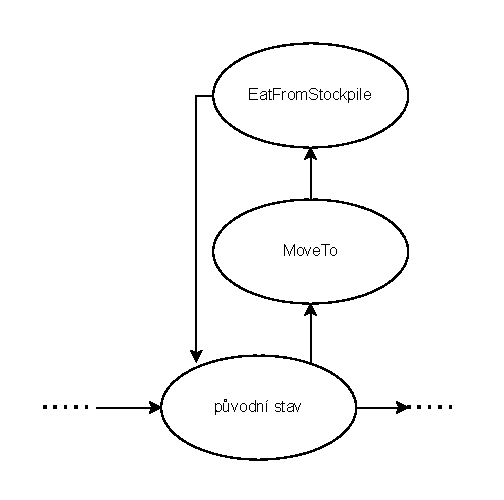
\includegraphics[width=0.6\linewidth]{img/transition.pdf}
    \caption{Řešení mechaniky hladu pro jeden vrchol z původního stavového automatu.}
    \label{fig:transition}
\end{figure}

Alternativní způsob by byl použít dva stavové automaty. Hlavním automatem by byl automat řešící hlad, který by měl \texttt{MainState} ve kterém by se nejprve zkontrolovalo zda hladovění vesničana nekleslo pod určitou hodnotou, pokud ne tak zavolá původní automat, jinak nastane přechod do již zmiňované dvojice stavů \texttt{MoveToState} a \texttt{EatFromStockpileState}.

Je lehké nahlédnout, že obě řešení přidávají netriviální složitost navíc do definice chování pro naše vesničany.

Podle výše zmíněného článku mají \textit{stromy chování} dobrou rozšiřitelnost a modularitu. Pokud bychom chtěli rozšířit náš \textit{strom chování} o výše zmíněnou mechaniku hladu, mohli bychom vytvořit nový strom chování, který by použil \texttt{Selector} vrchol jako kořen, který by měl dva potomky. Prvním by byl podstrom řešící mechaniku hladu a druhým by byl celí původní strom připojený kořenem jako podstrom nového stromu chování. Celá situace by vypadala takto:

\begin{verbatim}
    Builder.Create()
      .Selector("tree root")
        .Sequence("villager hunger sequence")
          .Condition("is hunger bellow threshold?", IsHungry)
          .Condition("is there food?", IsThereFood(stockpile))
          .Do("go to get food", MoveTo(stockpile))
          .Do("eat food", EatFood)
        .End()

        .Sequence("villager job sequence")
          // original tree as subtree
        .End()
      .End()
\end{verbatim}

Je lehké nahlédnout, že rozšiřitelnost a modularita \textit{stromů chování} jsou opravu silné vlastnosti. Proto také \textit{stromy chování} použijeme pro definici chování pro naše vesničany.


\section{Generovaný svět}
\label{sec:terrain}
Jak jsme si specifikovali v sekci~\ref{sec:game-world}, svět v naší hře bude náhodně generovaný. Konkrétně bude obsahovat náhodně generovaný terén ve kterém budou náhodně umístěny suroviny a vesnice.

Vygenerovaný terén bude 2D plocha, která se bude skládat ze spojitých oblastí. Každá oblast bude odpovídat nějakému biomu a bude mít barvu podle tohoto biomu (například oblast odpovídající biomu vody bude modrá). Některé oblasti mezi sebou budou mít závislosti (například oblast, která reprezentuje biom vysoké hory, bude obklopena oblastí, která reprezentuje biom hory). Je nutné zmínit, že nechceme políčka, ale opravdu spojité oblasti.

Naši hru budeme používat převážně pro měření výkonu ECS knihoven, tím pádem nemáme na generování našeho terénu žádné složité požadavky. Mezi naše požadavky patří:

\begin{enumerate}
    \item \textbf{Generování terénu by nemělo trvat příliš dlouho:} Pokud by generování terénu trvalo příliš dlouho, vedlo by to k delšímu času spouštění naší hry. Vzhledem k tomu, že hru budeme používat pro měření výkonu ECS knihoven a pro každou knihovnu ji pouštět znovu, delší čas spouštění hry by nám zbytečně natahoval dobu vykonávání jednoho měření.

    \item \textbf{Možnost navigace:} Ze sekce~\ref{subsec:villages} víme, že hra bude obsahovat vesničany. Pro vesničany bude důležité aby byli schopni se v náhodně vygenerovaném terénu navigovat. Pokud vesničan bude například chtít jít pokácet strom, bude se chtít po cestě k němu vyhnout vodě.

    \item \textbf{Žádné vizuální artefakty:} Chceme se vyhnout vizuálním artefaktům, díky kterým by náš terén nevypadal dobře.
\end{enumerate}

\subsection{Generování terénu}
\label{sec:terrain-gen}
Z požadavků na naši hru, které jsme si představili v sekci~\ref{sec:game-characteristics} vyplývá, že nechceme naši hru dělat příliš složitou. Terén tedy budeme generovat tím, že si za pomoci šumové funkce nejprve vytvoříme výškovou mapu a tu poté obarvíme. Tento přístup jsme zvoli jelikož je jednoduchý na implementaci a poskytuje dobře vypadající terén.

Pro vygenerování výškové mapy bude nejprve nutné zvolit šumovou funkci, proto si jednotlivé šumové funkce nejprve rozebereme:

\begin{enumerate}
    \item \textbf{Perlinův šum:} Jedná se o známou šumovou funkci. Tato šumová funkce je rychlá a také jednoduchá na implementaci. Je jí možné použít v libovolné dimenzi, ale nejčastěji se používá ve druhé nebo třetí. Přehledné vysvětlení o tom co to je Perlinův šum a jak se používá pro generování terénu je možné nalézt v diplomové práci \textit{Terrain synthesis using noise}~\cite{TerrainNoise} od \textit{Tuoma Hyttinena}.

    \item \textbf{Simplexový šum:} \textit{Simplexový šum} je velmi podobný \textit{Perlinovu šumu}. Přehledné vysvětlení o tom co to je \textit{Simplexový šum} a jak se používá pro generování terénu je možné nalézt v již zmíněné diplomové práci \textit{Terrain synthesis using noise}~\cite{TerrainNoise}. V této práci je možné se dočíst, že oproti \textit{Perinovu šumu} je \textit{Simplexový šum} rychlejší a produkuje výsledky, které vypadají více přirozeně. Ovšem má jednu velkou nevýhodu a to patent, který omezuje jeho použití pro komerční účely. Z toho důvodu se v praxi tolik nepoužívá.
\end{enumerate}

I přesto je \textit{Simplexový šum} nabízí výhody oproti \textit{Perlinovu šumu}, pro implementaci zvolíme \textit{Perlinův šum} z důvodů již zmíněného patentu. Konkrétně jej budeme používat ve druhé dimenzi.

Nyní za pomoci \textit{Perlinova šumu} vygenerujeme výškovou mapu. Pro generování výškové mapy lze použít Fraktální součet nebo TurbulencI. Jedná se o techniky pro generování více komplexních vzorů. O obou technikách je možné se více dočíst v již zmíněné diplomové práci \textit{Terrain synthesis using noise}~\cite{TerrainNoise}.

Pro zvolení techniky autor práce provedl experiment a nechal vygenerovat terén pomocí obou technik. Z výsledných terénů autor více preferoval terén vygenerovaný Fraktálním součtem, proto jej zvolíme.

Nyní zbývá pomocí výškové mapy vygenerovat daný terén. Již víme, že náš terén bude 2D plocha. Tuto plochu si rozdělíme na malé atomické části (například pixely) a těmto částem přiřadíme souřadnice. Barva každé části bude odpovídat danému biomu. Každý biom bude mít definovaný výškový interval a barvu. Pro souřadnice každé atomické části si necháme vygenerovat výšku z výškové mapy. Poté na základě této výšky a výškových intervalů jednotlivých biomů získáme příslušný biom. Poté barvu dané části nastavíme na barvu daného biomu. O této technice je možné se více dočíst ve článku \textit{Making maps with noise functions}~\cite{TerrainHeightMap} ze stránky \textit{Red Blob Games}.

Příklad výsledného terénu je možné vidět na obrázku~\ref{fig:terrain}.

\begin{figure}[!htb]
    \centering
    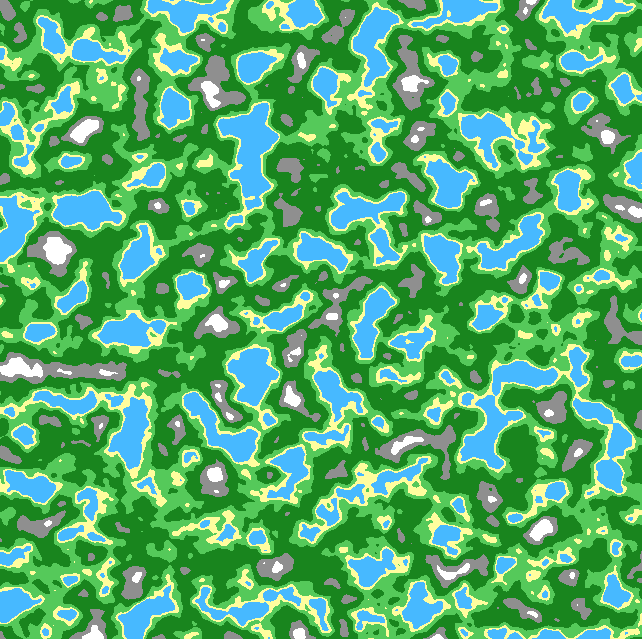
\includegraphics[width=0.66\linewidth]{img/terrain.png}
    \caption{Příklad jak může vypadat námi vygenerovaný terén.}
    \label{fig:terrain}
\end{figure}

\subsection{Generování terénu na CPU vs. GPU}
Za použití techniky z minulé sekce jsme získali vygenerovaný terén. Ovšem to jestli naše technika splňuje naše požadavky je závislé na tom zda terén budeme generovat na CPU nebo na GPU. Proto si nyní oba přístupy rozebereme.

\subsubsection{Generování terénu na CPU}
Při generování terénu na CPU bychom si pořídili jednu nebo více textur a vygenerovali terén v nich za použití způsobu z minulé sekce.

Při generovaní tohoto terénu je možné zvolit rozlišení, konkrétně specifikaci velikosti atomických částí. Volba tohoto rozlišení nám ovlivňuje dobu trvání vygenerování našeho terénu. Pokud bychom zvolili malé atomické části, generování by trvalo příliš dlouho a porušili bychom požadavek na rychlost. Pokud bychom zvolili velké atomické části, generování by trvalo menší dobu, ale zase bychom porušili požadavek na absenci vizuálních artefaktů.

V ideálním případě bychom chtěli velké rozlišení ale také lepší rychlost. Jeden ze způsobů jak toho dosáhnout je paralelizace, ovšem možnosti paralelizace na CPU jsou oproti GPU omezeny, proto si rozeberme jak by se dal terén generovat na GPU.

\subsubsection{Generování terénu na GPU}
Terén budeme generovat v reálném čase (vygenerujeme jej v každém snímku znova) a vždy nám postačí vygenerovat pouze část terénu, která je viditelná hráčem. Tato část bude bude obdélník se stejnými rozměry jako velikost okna naší hry.

Pořídíme si texturu do které budeme generovat terén. Tato textura bude mít stejnou velikost jako okno naší hry. Poté si pořídíme fragment shader, kterým do této textury budeme generovat terén. Tento fragment shader v každém snímku na základě pozice a přiblížení kamery pro každý pixel naší textury provede algoritmus popsaný v sekci~\ref{sec:terrain-gen}.

Díky vysoké paralelizaci GPU můžeme vždy zvolit nejmenší velikost atomických oblastí (velikost jednoho pixelu) a stejně budeme mít pořád dostatečnou rychlost.

\subsection{Navigace ve vygenerovaném terénu}
Generování terénu na GPU se zdá být ideálním kandidátem, ovšem tím, že terén budeme generovat na GPU, nám vzniká problém, jak ve vygenerovaném terénu budeme vlastně provádět navigaci. V této sekce tento problém vyřešíme.

Vesničané v naší hře budou často potřebovat nalézt cestu v námi vygenerovaném terénu k nějaké entitě. Budou například chtít dojít ke skladišti nebo ke svému pracovnímu místu. Jelikož k hledaní cesty bude docházet poměrně často budeme chtít aby bylo dostatečně rychlé. Dále budeme chtít, aby cesty působily přirozeně. Příklady vhodných (přirozených) a nevhodných (nepřirozených) cest je možné vidět na obrázku~\ref{fig:path}.

\begin{figure}[!htb]
    \centering
    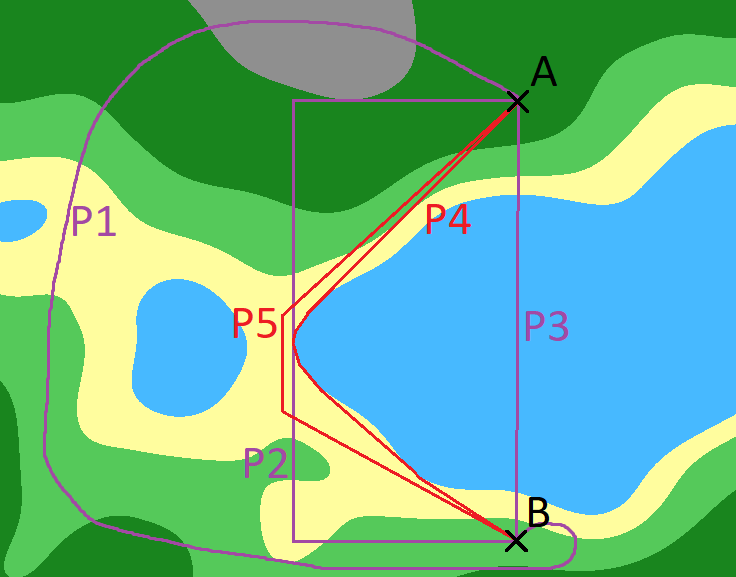
\includegraphics[width=0.66\linewidth]{img/path.png}
    \caption{Příklad cest z bodu A do bodu B. Fialové cesty jsou nevhodné. Červené cesty jsou vhodné.}
    \label{fig:path}
\end{figure}

Fialové cesty jsou nevhodné. Konkrétně cesta $P1$ je nevhodná, jelikož vede zbytečnou velkou oklikou. Cesta $P2$ je nevhodná, protože vede pouze podel os. Cesta $P3$ je nevhodná, jelikož vede přes vodu.

Červené cesty jsou vhodné. Cesta $P4$ je nejkratší cestou z bodu $A$ do bodu $B$. Cesta $P5$ sice není nejkratší cesta ale je pro nás dostatečně dobrou aproximací a je pro nás dostačující.

\subsubsection{Navigační struktury}
Pro navigaci v terénu použijeme datovou strukturu. Tato datová struktura reprezentuje terén způsobem, který umožňuje snadné hledaní cest mezi dvěma body. Často k tomu používají algoritmus pro hledání nejkratších cest. Typickou volbou bývá algoritmus A*. Datové struktury, které lze pro navigaci použít nazvěme navigační struktury.

Velkou část navigačních struktur tvoří navigační meshe (nebo také zkráceně navmesh). Ty jsou často používány populárními frameworky a enginy jako je například Unity. Navigační meshe vezmou plochu terénu po které lze chodit a rozdělí ji do oblastí. Každá taková oblast je tvořena konvexním polygonem. Poté si vytvoří graf, kde každý takovýto polygon je reprezentován vrcholem a každé sousední polygony mají mezi sebou hranu. V tomto grafu se poté hledají nejkratší cesty. Je nutné upozornit, že existuje velké množství navigačních meshů a některé se od tohoto popisu mouhou lišit. Pro více informacích o navigačních meshích lze nahlédnou do studie \textit{A comparative study of navigation meshes}~\cite{10.1145/2994258.2994262}.

V sekci~\ref{sec:game-characteristics} jsme si uvedli, že nechceme aby naše hra byla příliš složitá, jelikož by to odvádělo pozornost od problému, který řešíme. Z toho důvodu nebudeme používat navigační mesh jako navigační strukturu pro naši hru, jelikož i přesto, že použití navigačního meshe pro navigaci není složitá úloha tak jeho konstrukce složitá já.

Jako navigační strukturu zvolíme dvourozměrnou mřížku. Tu si budeme reprezentovat jako pole, kde každý prvek tohoto pole ponese informaci o tom v jakém biomu se nachází daný vrchol mřížky. Tuto strukturu zvolíme, protože je jednoduchá na konstrukci. Cesty které díky této mřížce získáme nebudou nejlepší možnou nejkratší cestou (a nebudou ve skutečnosti ani nejkratší), ale budou pro nás dostatečně dobrou aproximací. 

\subsubsection{Tvorba cesty}
Tvorbu cesty začneme tím, že získáme cestu, která se bude z počátku nevhodná. Poté ji vylepšíme a tím získáme cestu, která již bude vhodná.

Pro výpočet vzdálenosti mezi dvěma body v naší mřížce zvolíme Manhattanskou metriku. Pro hledání nejkratších cest použijeme algoritmus A*. První tvar naší cesty získáme tím, že pomocí A* algoritmu nalezneme cestu v naší mřížce. Příklad toho jak by taková cesta mohla vypadat je možné vidět na obrazku~\ref{fig:path_grid}. Je lehké nahlédnout, že se podobá cestě $P2$ z obrázku~\ref{fig:path}, která je pro nás nevhodná.

\begin{figure}[!htb]
    \centering
    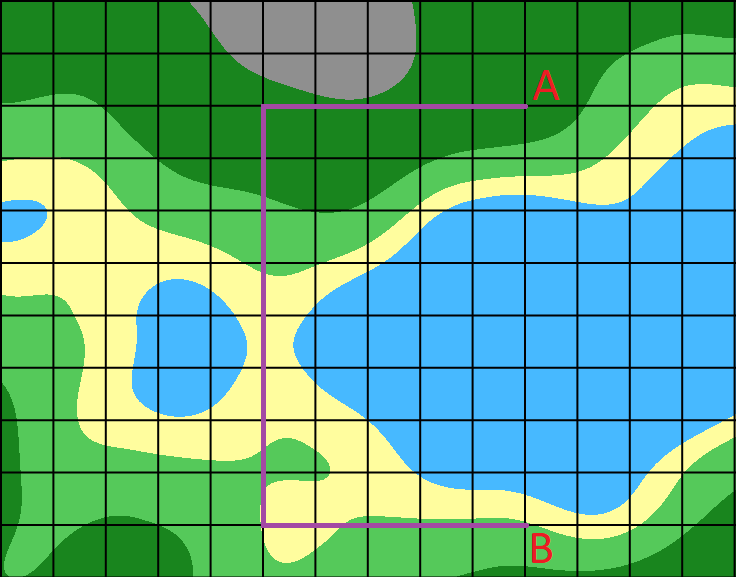
\includegraphics[width=0.66\linewidth]{img/path_grid.png}
    \caption{Příklad cesty z bodu A do bodu B nalezené A* algoritmem v naší mřížce.}
    \label{fig:path_grid}
\end{figure}

Následně provedeme úpravu této cesty.Začneme v prvním bodu cesty a provedeme ray cast do druhého bodu. Pokud jsme nenarazili na vodu pokusime se provést ray cast ke třetímu bodu. To budeme opakovat dokud náš ray cast nenarazil na vodu. V takovém případě můžeme cestu zjednodušit a odstranit z ní všechny body mezi prvním a posledním úspěšným. Poté ce přesuneme ke druhému bodu a postup opakujeme. Celí tento proces provádíme dokud nedojdeme do posledního bodu naší cesty. Zjednodušení fialové cesty je možné vidět na obrázku~\ref{fig:path_simplified}, kde fialová cesta představuje původní cestu a červená cesta její zjednodušení.

\begin{figure}[!htb]
    \centering
    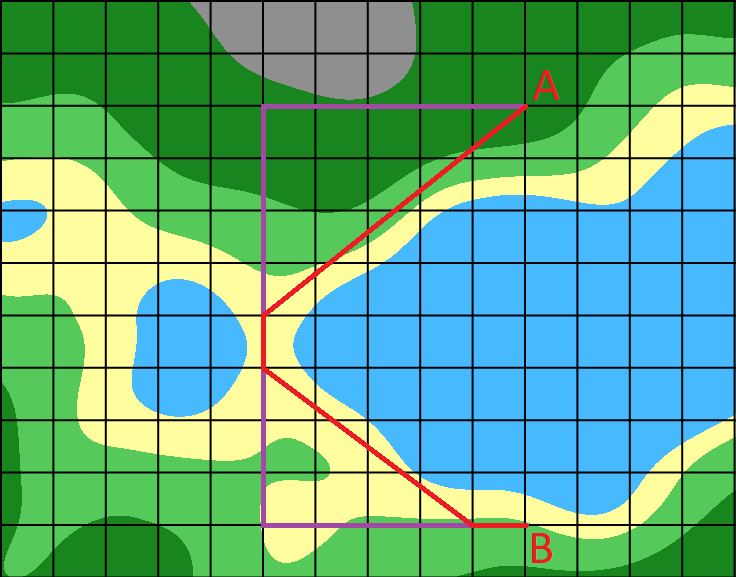
\includegraphics[width=0.66\linewidth]{img/path_simplified.png}
    \caption{Příklad cesty z bodu A do bodu B nalezené A* algoritmem v naší mřížce, která byla následně zjednodušena. Fialová cesta je originální nevhodná cesta. Červená cesta je zjednodušená, již vhodná, cesta.}
    \label{fig:path_simplified}
\end{figure}

Ovšem problém spočívá v tom, že k dispozici máme pouze mřížku, která obsahuje data o našem terénu, tím pádem nemůžeme provést klasický ray cast. Proto provedeme pouze jeho aproximaci. Začneme v bodu $N$ a chceme provést aproximaci ray castu do bodu $M$. Spočítáme si směr z bodu $N$ do bodu $M$ a tímto směrem se budeme posouvat vždy o nějakou malou vzdálenost $\Delta$. Pokaždé když se posuneme tak si spočítáme nejbližší bod z naší mřížky. Pokud se jedná o bod s biomem vody, tak ray cast selhal. V případě, že jsme takto došli až do bodu $M$ a nenarazili jsme na bod vody, ray cast byl úspěšný.

Mohlo by se zdát, že použití této aproximace by vedlo v příliš nevhodné cesty, ovšem za předpokladu, že se body v naší mřížce budou nacházet dostatečně blízko sebe, tak bude výsledná cesta dostatečně dobrou aproximací červené cesty z obrázku~\ref{fig:path_simplified}.

Další problém, který je nutné vyřešit, je, že vesničané a entity, ke kterým se vesničané navigují, nejsou umístěni v naší mřížce. Problém vyřešíme tak, že před spuštěním A* algoritmu si k vesničanovi a dané entitě nalezneme nejbližší body v naší mřížce a nalezneme nejkratší cestu mezi těmito body. Poté, předtím než provedeme zjednodušení cesty, přidáme pozici vesničana jako první bod naší cesty a pozici entity, ke které se vesničan naviguje, jako poslední bod naší cesty. Přidáním těchto bodů by nám mohli vzniknout nepřirozené artefakty, ovšem ty budou spraveny během zjednodušování cesty.

Zbývá nám vyřešit jak získáme již zmiňovanou mřížku. Abychom ji získali z našeho terénu bude potřeba jej navzorkovat. Podobně jako při jeho generování si terén rozdělíme na atomické části a střed každé takové atomické části bude bodem v naší mřížce. Protože celý náš terén generujeme na GPU, bude nutné toto navzorkování také provádět na GPU. Pořídíme si proto compute shader pomocí kterého terén navzorkujeme na GPU a tím vytvoříme mřížku, kterou poté přesuneme na CPU.

Ovšem problém nastává v tom, že MonoGame framework, který pro tvorbu naší hry používáme nemá podporu pro compute shadery. Z toho důvodu namísto nativního MonoGame zvolíme jeho fork~\cite{MonoGameCptMax} od Markuse Hötzingera, který tuto podporu přináší.

\section{Měření}
Z úvodu této kapitoly víme, že náš projekt je reprezentován C\# řešením. Toto C\# řešení se skládá ze dvou C\# projektů a to hry a poté měření, které používá onu hru pro měření výkonu ECS knihoven. V této sekci se budeme věnovat analýze tohoto měření.

\subsection{Jak budeme měření provádět}
Prvně si přiblížíme co to je \textit{game loop}, jelikož to budeme potřebovat k popisu měření. Následně si popíšeme samotné měření.

\subsubsection{Game loop}
\textit{game loop} si můžeme představit jako cyklus, který běží dokud nedojde k ukončení hry. Pseudokód pro \textit{game loop} může vypadat například takto:

\begin{verbatim}
    while (!shouldExit) 
    {
      Update();
      Draw();
    }
\end{verbatim}

Pseudokód obsahuje \texttt{while} cyklus, který se opakuje dokud nedojde k nastavení proměnné \texttt{shouldExit} na \texttt{true}. V těle tohoto cyklu se volají dvě funkce a to \texttt{Update}, která je zodpovědná za zpracování herní logiky a \texttt{Draw}, která je zodpovědná za vykreslení hry. 

I naše hra obsahuje \textit{game loop}. Logika v naší hře se skládá ze systémů. Ty se dělí na \textit{update systémy}, které řeší zpracování herní logiky a \textit{render systémy}, které řeší vykreslování. \textit{Update systémy} běží uvnitř funkce \texttt{Update} a \textit{render systémy} běží uvnitř funkce \texttt{Draw}. Je nutné upozornit, že tento popis je zjednodušen a více dopodrobna se implementaci hry a systémů budeme věnovat v následující kapitole.

\subsubsection{Popis měření}
Budeme mít stanovené dva pevné počty iterací. První bude přípravný počet iterací a druhý bude měřený počet iterací. Měřený počet iterací bude větší než přípravný počet iterací.

Samotné měření se bude skládat ze dvou fází a to fáze přípravy a fáze měření. Během fáze přípravy vytvoříme instanci naší hry s konkrétní ECS knihovnou a necháme její \textit{game loop} běžet přípravný počet iterací. Během fáze měření vezmeme tu samou instanci hry, která běžela přípravný počet iterací a necháme její \textit{game loop} běžet měřený počet iterací. Během fáze měření budeme také měřit čas, během kterého hra provádí měřený počet iterací svého \textit{game loop}. Tento čas bude výsledným časem pro jednu konkrétní ECS knihovnu.

Výše popsaný test provedeme pro každou ECS knihovnu, kterou budeme měřit. Pomocí výsledných časů můžeme relativně porovnat výkon naší hry s různými ECS knihovnami. 

Při měření výkonu jednotlivých ECS knihoven ignorujeme některé jejich funkcionality. Konkrétně se jedná o funkcionality rozšíření ECS. Jedná se například o funkcionality známe pod názvy \textit{reakční systémy} (\textit{reaction systems}) nebo \textit{relace} ({\textit{relations}}). V našem měření je budeme ignorovat protože chceme měřit klasické ECS bez rozšířeních.

\subsection{Volba frameworku pro měření}
Nyní zvolíme framework, který budeme používat pro měření. Prvně si popíšeme vlastnosti, kterého od tohoto frameworku požadujeme, poté provedeme samotný výběr. Mezi požadované vlastnosti patří:

\begin{enumerate}
    \item \textbf{Korektnost:} Chceme aby naměřené výsledky byli spolehlivé. Klíčovým faktorem bude aby výsledek vyprodukovaný pro danou ECS knihovnu byl porovnatelný s výsledkem vyprodukovaným pro jinou ECS knihovnu.
    \item \textbf{Jednoduchost:} Budeme chtít aby framework byl jednoduchý na používání. Nechceme dávat přednost jednoduchosti před korektností, ale pokud bude na výběr mezi frameworky co splňují první požadavek, tak upřednostníme ten, který je jednodušší na používání.
\end{enumerate}

Pro výběr frameworku použijeme platformu GitHub. Na stránce~\cite{github_performance} je možné vidět seznam repositářů na platformě GitHub s topicem \textit{performance} seřazené podle počtu hvězd. Je možné nahlédnou, že nejpopulárnějším frameworkem pro měření výkonu je \textit{BenchmarkDotNet}~\cite{BenchmarkDotNet}.

\textit{BenchmarkDotNet} je framework pomocí kterého lze měřit výkon metody. Tento framework splňuje oba naše požadavky, ale jedná se o framework primárně určený na micro benchmarky, zatímco naše měření je spíše macro benchmarkem. I přesto jej pro naše měření použijeme, primárně protože je velmi jednoduchý na použití.

















% \subsection{Jak lze měřit výkon hry}
% Pro měření výkonu budeme mít test, který si pro každou ECS knihovnu, kterou budeme měřit, vytvoří novou instanci naší hry běžící s danou ECS knihovnou. Poté tento test změří výkon každé takovéto instance. Ještě předtím, než si rozebereme přístupy pro měření výkonu hry si nejprve připomeneme co to je \textit{game loop}.

% \subsubsection{Game loop}
% \textit{game loop} si můžeme představit jako cyklus, který běží dokud nedojde k ukončení hry. Pseudokód pro \textit{game loop} může vypadat například takto:

% \begin{verbatim}
%     while (!shouldExit) 
%     {
%       Update();
%       Draw();
%     }
% \end{verbatim}

% Pseudokód obsahuje \texttt{while} cyklus, který se opakuje dokud nedojde k nastavení proměnné \texttt{shouldExit} na \texttt{true}. V těle tohoto cyklu se volají dvě funkce a to \texttt{Update}, která je zodpovědná za zpracování herní logiky a \texttt{Draw}, která je zodpovědná za vykreslení hry. 

% I naše hra obsahuje \textit{game loop}. Logika v naší hře se skládá ze systémů. Ty se dělí na \textit{update systémy}, které řeší zpracování herní logiky a \textit{render systémy}, které řeší vykreslování. \textit{update systémy} běží uvnitř funkce \texttt{Update} a \textit{render systémy} běží uvnitř funkce \texttt{Draw}. Je nutné upozornit, že tento popis je zjednodušen a více dopodrobna se implementaci hry a systémů budeme věnovat v následující kapitole.

% \subsubsection{Přístupy k měření výkonu}


% Nyní si rozebereme přístupy, kterými lze měřit výkon naší hry.

% co si od toho predstavujeme, jak to chceme delat

% vyber frameworku pro mereni

% na co nebudeme brat ohledy a proc









% První si popíšeme kde tuto mřížku vezmeme a poté jak ji budou využívat vesničané pro navigaci.

% Abychom získali z našeho terénu mřížku bude třeba jej navzorkovat. Podobně jako při jeho generování si terén rozdělíme na atomické části a střed každé takové atomické části bude bodem v naší mřížce. Ovšem celý náš terén generujeme na GPU, proto toto navzorkování bude nutné také provést na GPU. Pořídíme si proto compute shader pomocí kterého terén navzorkujeme na GPUa tím vytvoříme mřížku, kterou poté stáhneme do CPU.

% Ovšem problém nastává v tom, že MonoGame framework, který pro tvorbu naší hry používáme nemá podporu pro compute shadery. Z toho důvodu namísto nativního MonoGame zvolíme jeho fork~\cite{MonoGameCptMax} od Markuse Hötzingera, který tuto podporu přináší.




% \xxx{TODO: path-finding}

% Naše hra bude obsahovat procedurálně generovaný terén. Ten je možné generovat pomocí CPU nebo pomocí GPU. Obě možnosti si nyní rozebereme.

% % \subsubsection{Generování terénu na CPU}
% Při generování terénu na CPU nám postačí terén vygenerovat pouze jednou při spuštění hry a výsledek si poté uložit do jedné nebo více textur. Tento přístup má ale dva problémy. Prvním problémem je, že pokud dojde k většímu přiblížení nebo oddálení kamery, dojde k deformaci těchto textur. To může způsobit různé vizuální artefakty. Druhým problémem je, že vytváření zmíněných textur může trvat delší dobu. To může vést k delšímu času spouštění hry.

% % \subsubsection{Generování terénu na GPU}
% Pro vygenerování terénu na GPU ja potřeba vytvořit shader. Tento shader vezme pozici a přiblížení kamery a vygeneruje pro tyto parametry terén. Díky vysoké paralelizace na GPU můžeme terén generovat za běhu. Při generování terénu za běhu nám nevzniknou výše zmíněné vizuální artefakty. Vyřeší se nám i druhý problém, jelikož nemusíme čekat na vygenerování výše zmíněné textury.

% Je snadné nahlédnout, že generování terénu na GPU je pro nás výhodnější, proto tento přístup zvolíme.

% \section{Hledání cesty ve vygenerovaném terénu}
% \label{subsection:path-finding}
% Vesničané musejí často vyhledávat cestu z bodu A do bodu B. Například potřebují dojít ke svému pracovnímu místu, nebo odnést předmět do skladiště.

% V případě generování terénu na CPU by bylo hledání cesty velice jednoduché. Stačilo by nám vzít vygenerovanou texturu a najít danou cestu v ní. Ovšem problém spočívá v tom, že terén generujeme pomocí GPU a vyhledávání cesty musíme vykonávat na CPU.

% Pro řešení problému s hledáním cesty si zavedeme \textit{compute shader}, který jako vstupní parametr přijme rozlišení. Výstupem tohoto \textit{compute shaderu} bude dvourozměrné pole sestavené z nevzorkovaného terénu při daném rozlišení. Tento \textit{compute shader} nám tedy při spuštění hry vytvoří dvourozměrné pole na GPU, to si poté stáhneme na CPU a v něm poté můžeme provádět vyhledávání cesty.

% Chceme pěkné cesty, takže výslednou cestu zkrášlujeme.

% Generování může trvat, protože přesun dat mezi GPU a CPU je drahý.

% Je nutné použít fork MonoGame, který podporuje compute shadery.

% \section{Owner komponenta}
% Při práci s ECS je někdy potřeba získat identifikátor příslušné entity. Ovšem v kontextu systému, který pouze iteruje přes komponenty na jednotlivých entitách to může být problematické.

% Řešení, které některé ECS knihovny nabízejí je možnost iterovat identifikátory entit společně s jejich komponentami. Ovšem ne každá ECS knihovna to umí, proto je potřeba zvolit jiný přístup.

% Přístup, který jsme zvolili je zavedení \texttt{Owner} komponenty. Jednotlivé entity jsou v naší hře reprezentovány třídou dědicí od \texttt{IEntity}. \texttt{Owner} komponenta má pouze jeden jediný člen a to referenci na \texttt{IEntity}, která představuje jejího majitele.









% \subsection{Reprezentace systémů}
% Jak již bylo zmíněno v úvodu, velký problém při návrhu systémů je rozdílné rozhrani, které pro systémy jednotlivé ecs knihovny nabízejí.

% Dále, jak již jsme si zmiňovali v podkapitole o herních požadavcích, chceme aby se výkon naší hry při použití této abstrakční vrstvy blížil výkonu s použitím pouze samotné ecs knihovny.

% Nahlédneme na oba tyto problémy blíže a prozkoumáme jak jsme je vyřešili.

% \subsubsection{Rozhraní ecs knihoven}
% ECS knihovny reprezentují systémy následujícími způsoby:

% \begon{ordering}
% \item \xxx{TODO}
% \end{ordering}











% V této sekci si představíme knihovny, které budeme chtít měřit. Nahlédneme na jejich rozhraní a na základě toho odůvodníme rozhodnutí provedené při implementaci abstrakční vrstvy.

% % - knihovny
% \subsection{Měřené knihovny}
% Než začneme provádět analýzu abstrakční vrstvy, musíme si nejprve představit jednotlivé knihovny, které budeme chtít měřit. Následně nahlédneme na jejich rozhraní, to nám pomůže při analýze abstrakční vrstvy.

% % --- predstaveni knihoven
% I přesto, že lze program použít pro měření velkého množství ECS knihoven pro C\#, omezíme se pouze na následující:

% \begin{enumerate}
%     \item Arch~\cite{Arch}
%     \item DefaultEcs~\cite{DefaultEcs}
%     \item Entitas~\cite{Entitas}
%     \item HypEcs~\cite{HypEcs}
%     \item LeoECS~\cite{LeoECS}
%     \item \xxx{Pridat dalsi knihovny kdyz bude cas.}
% \end{enumerate}

% \xxx{ --- rozebrat interface knihoven}\\\\

% \section{Inline entity processor}

% Inlinování funkcí je optimalizace, při které je volání funkce nahrazeno jejím obsahem.

% % priklad, kdy dochazi k inlinovani

% Kvůli měření je důležité, aby naše entity procesory neměli ideálně žádný overhead.

% Pro inlinování entity procesorů, využíváme následující techniky.

% % aggressive inlining, struktura + generika

% % \\
% % \xxx{Proc je to potreba}
% % \\
% % \xxx{Jak jsme toho dosahli}
% % \\

% \xxx{ - entity processor}\\\\
% \xxx{ --- -> entity processor}\\\\
% \xxx{ --- co je inline function call}\\\\
% \xxx{ --- jak jej zaridit}\\\\
% \xxx{ --- -> proto struktura a generika (IECSSystem)}\\\\

% \xxx{ - IEntity (chceme bohate rozhrani, jak jsme si popisovali)}\\\\
% \xxx{ - IWorld (nektere ECS knihovny potrebuji Update/Tick)}\\\\
% \xxx{ - Component attribute}\\\\
% \xxx{ - ECSFactory (proc types - zjednoduseni rozhrani)}\\\\

% \section{Analýza hry}

% text

% \subsection{Implementace AI}

% Nyní si rozebereme populární přístupy pro implementaci AI ve hrách.

% Nejpřímočařejší způsob je použít stavové automaty.

% Pokročilejší zpusob jsou behavior trees.

% Další pokročilejší způsob je Goal Oriented Action Planning (GOAP).

% Proč jsme zvolili behavior trees?

% Chování AI agentů může být popsané také přímo v systémech.

% Ne vždy je zřejmé co by mělo být součástí AI.

% \\
% \xxx{jaka jsou mozsnosti?}
% \\
% \xxx{- behavior trees}
% \\
% \xxx{- state machines}
% \\
% \xxx{- GOAP}
% \\
% \xxx{proc jsme zvolili behavior trees?}
% \\
% \xxx{behavior primo v systemech a proc jsme to nepouzili}
% \\
% \xxx{Co by melo byt rizeno AI a co ne?}
% \\
% \xxx{- tezba surovin: pripsani do inventare vs damage and drop system}
% \\
% \xxx{- zpracovani surovin: pripsani do inventare vs resource processing system}
% \\

% \subsection{ECS}

% Některé systémy v ECS reagují pouze pokud je pro danou entitu splněna určitá podmínka.

% Na první pohled by se mohlo zdát, že jsou tyto systémy špatné, jelikož podmínka je drahá operace.

% Alternativní a pravděpodobně lepší způsob je použít eventy.

% Rozeberme si jak by se s eventy v ECS pracovalo.

% Další způsob, jak by se tento problém dal řešit jsou Reaction systémy.

% \\
% \xxx{condition checking systems are ok}
% \\
% \xxx{eventy v ECS}
% \\

% \subsection{Generovani terenu}

% Rozeberme si dva přístupy pro generování terénu.

% První způsob je generovat terén přímo na CPU.

% Druhý způsob je pro generování terénu použít GPU.

% problem s path finding

% Abychom si rozebrali řešení, bude nejprve nutné nejprve  něco více o shaderech.

% Compute shader můžeme použít k řešení výše zmíněného problému.

% \xxx{GPU vs CPU}
\chapter{Popis implementace}
V této kapitole si představíme klíčové a zajímavé části implementace. Pro více detailů o implementaci je možné nahlédnout do kódu, který obsahuje dokumentační komentáře.

Pro celý projekt používáme jedno C\# solution. To obsahuje dva C\# projekty. Prvním je hra (\texttt{WorldSimulator.csproj}) a druhým je měření (\texttt{WorldSimulator.Benchmarks.csproj}), které používá vytvořenou hru pro měření výkonu ECS knihoven. Projekt hry se skládá ze tří částí. První částí jsou implementace ECS knihoven, které implementují abstrakční vrstvu. Nad nimi je samotná abstrakční vrstva, která je druhou částí. Třetí částí je hra samotná, která namísto konkrétní ECS knihovny používá abstrakční vrstvu.

\section{Abstrakční vrstva}
\label{sec:abstract-layer}
Abstrakční vrstva se nachází v jmenném prostoru \texttt{WorldSimulator.ECS.AbstractECS}. V jmenném prostoru \texttt{WorldSimulator.ECS} kromě abstrakční vrstvy lze také nalézt jednotlivé její implementace.

\subsection{Systémy}
V ECS jsou systémy zodpovědné za iterace a zpracování entit. Jelikož každá ECS knihovna iteruje přes entity jiným způsobem, a zároveň chceme definovat zpracování entit (herní logiku) pouze jednou, bude nutné implementaci rozdělit do několika tříd. Vztah tříd, které souvisejí se systémy, je možné vidět na obrázku~\ref{fig:abstract-layer-systems}.

\begin{figure}[!htb]
  \centering
  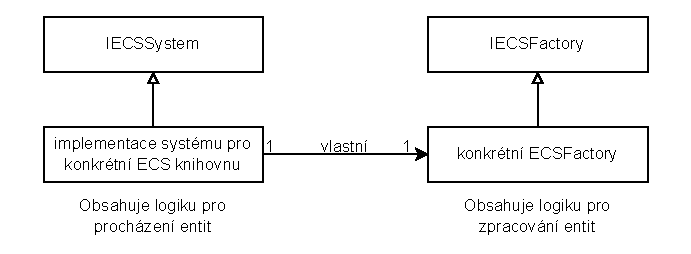
\includegraphics[width=0.8\linewidth]{img/abstract-layer-systems.pdf}
  \caption{Vztahy tříd souvisejících se systémy.}
  \label{fig:abstract-layer-systems}
\end{figure}

\texttt{IECSSystem} je rozhraní, ze kterého dědí každý systém. Každá ECS knihovna poté poskytne svou implementaci systému. Tyto implementace obsahují pouze logiku pro iteraci neboli procházení přes jednotlivé entity. Každá implementace systému bude vlastnit konkrétní \texttt{EntityProcessor} dědicí od \texttt{IEntityProcessor}. Jednotlivé \texttt{EntityProcessor} jsou zodpovědné za zpracování entit. Jednotlivé implementace rozhraní \texttt{IECSSystem} jsou generické typy, které přijímají typ entity procesoru a také typy komponent, které od entit vyžadují jako generické parametry.

Jako příklad si uvedeme třídu \texttt{ArchSystem<TEntityProcessor, TComponent>}. Jedná se o implementaci systému. Tento systém obsahuje logiku pro iteraci entit z ECS knihovny \textit{Arch}~\cite{Arch}. Příkladem konkrétního \texttt{EntityProcessor} je například třída \texttt{MovementSystem}, která řeší zpracování entit s komponentami \texttt{Position} a \texttt{Movement} a obsahuje logiku zodpovědnou za jejich pohyb.

Z pohledu hry jednotlivé implementace \texttt{EntityProcessor} představují samotné systémy, jelikož hra nekouká na to, jak jsou entity iterovány, a zajímá jí jenom samotná herní logika. Proto se kód, který pracuje s hrou, odkazuje na \texttt{EntityProcessor} jako na systém. Ovšem z pohledu abstrakční vrstvy je nutné rozlišovat \texttt{System} jako typ, který obsahuje logiku pro iteraci entit, a \texttt{EntityProcessor} jako typ, který obsahuje logiku pro zpracování entit. Autor si je vědom, že tyto pohledy mohou vést k matoucí terminologii, ovšem v kódu jsou již používány na příliš mnoho místech.

\subsection{ECSFactory}
\texttt{ECSFactory} je abstraktní třída. Typy, které z ní dědí, jsou zodpovědné za tvorbu instancí souvisejících s abstrakční vrstvou. Vztah typů souvisejících s \texttt{ECSFactory} je možné vidět na obrázku~\ref{fig:abstract-layer-ecsfactory}.

\begin{figure}[!htb]
  \centering
  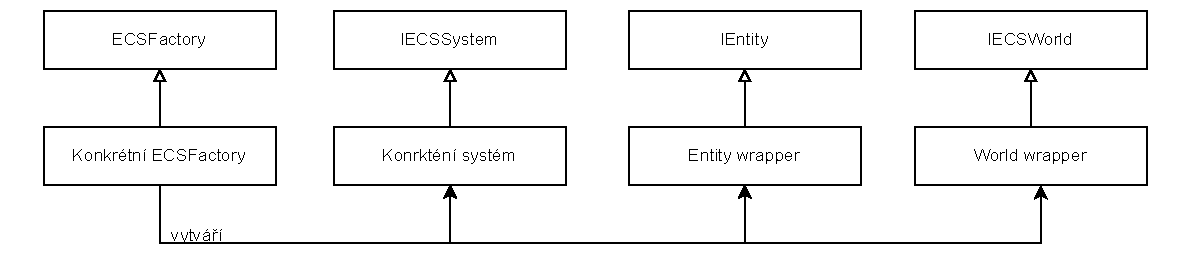
\includegraphics[width=1.0\linewidth]{img/abstract-layer-ecsfactory.pdf}
  \caption{Vztahy tříd souvisejících s \texttt{ECSFactory}.}
  \label{fig:abstract-layer-ecsfactory}
\end{figure}

Typ, který dědí od \texttt{ECSFactory}, musí implementovat metody pro vytváření instancí wrapperu entity a wrapperu \textit{worldu}. Skrze konstruktor svému předku také předá typy jednotlivých systémů (tříd dědicích od \texttt{IECSSystem}). Wrapper entity je třída dědicí od rozhraní \texttt{IEntity} a je zodpovědná za přidávání a odebírání komponent na dané entitě. Wrapper \textit{worldu} je třída dědicí od rozhraní \texttt{IECSWorld}. Tento wrapper implementuje metodu \texttt{Update}, která je zodpovědná za aktualizaci stavu \textit{worldu}.

\section{Hra}
\label{sec:game-impl}
Celá hra je reprezentována třídou \texttt{Game}, té je skrze konstruktor předána konkrétní instance \texttt{ECSFactory}. Jednotlivé instance \texttt{ECSFactory} reprezentují jednotlivé ECS knihovny, a volba této instance představuje volbu ECS knihovny, se kterou bude hra pracovat.

První herní stav je hře předán skrze metodu \texttt{SwitchState}. Samotná hra je spuštěna metodou \texttt{Run}.

\subsection{Herní stavy}
Celá hra se může skládat z několika herních stavů. Každý herní stav je reprezentován třídou dědicí od \texttt{GameState} a představuje herní obrazovku. Hra momentálně obsahuje pouze herní stav \texttt{LevelState}, který reprezentuje herní obrazovku obsahující gameplay, ale díky abstrakci herních stavů by bylo snadné ji rozšířit například o herní obrazovku herního menu nebo herní obrazovku s nastavením hry. Vztahy tříd souvisejících s třídou \texttt{GameState} lze vidět na obrázku~\ref{fig:game-state}.

\begin{figure}[!htb]
  \centering
  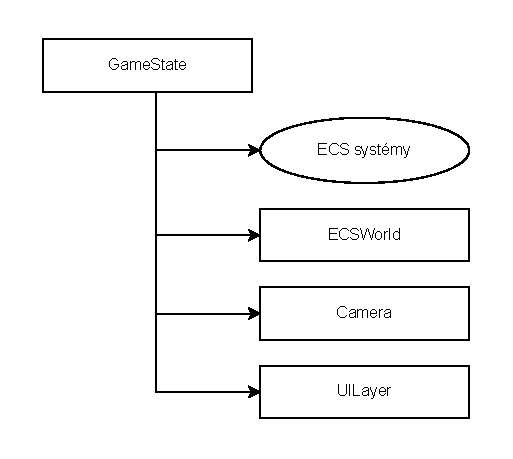
\includegraphics[width=0.5\linewidth]{img/game-state.pdf}
  \caption{Vztahy tříd souvisejících s \texttt{GameState}.}
  \label{fig:game-state}
\end{figure}

Každý herní stav obsahuje svoji instanci \texttt{ECSWorld}, která reprezentuje \textit{world} herního stavu. Tím pádem každý herní stav má svoji množinu entit. Dále má každý herní stav svoje systémy, kameru a instanci třídy \texttt{UILayer}, která spravuje prvky uživatelského rozhraní pro daný herní stav. Konkrétní herní stavy (instance tříd dědicích od \texttt{GameState}) jsou zodpovědné za vytváření svých entit, systémů a prvků uživatelského rozhraní.

V jeden moment může být aktivní pouze jeden herní stav. Ten lze zvolit za pomoci metody \texttt{SwitchState} na třídě \texttt{Game}. Vždy jsou aktivní pouze systémy v aktivním herním stavu.

\subsection{LevelState a herní svět}
\texttt{LevelState} je herní stav, který reprezentuje herní obrazovku obsahující samotný gameplay. Obrázek~\ref{fig:level-state} popisuje vztahy na této třídě.

\begin{figure}[!htb]
  \centering
  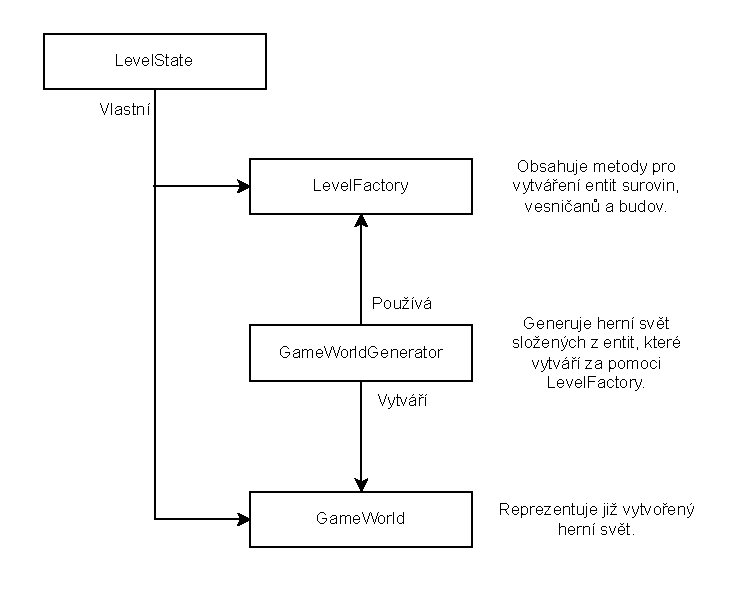
\includegraphics[width=0.7\linewidth]{img/level-state.pdf}
  \caption{Vztahy tříd souvisejících s \texttt{LevelState}.}
  \label{fig:level-state}
\end{figure}

Třída \texttt{LevelFactory} obsahuje metody pro vytváření entit surovin, budov a vesničanů. Tu využívá třída \texttt{GameWorldGenerator} pro tvorbu entit, ze kterých generuje herní svět. Ta se krom vytváření samotného terénu stará také a počáteční rozpoložení surovin a vesnic. Výsledný vygenerovaný herní svět je poté reprezentován třídou \texttt{GameWorld}.

Pomocí třídy \texttt{GameWorld} lze získávat informace o herním světě. Je možné nalézt nejbližší surovinu určitého typu k dané pozici, nalézt cestu mezi dvěma body nebo získat informace o terénu na dané pozici.

Na obrázku \ref{fig:game-world} lze vidět, že \texttt{GameWorld} obsahuje kd-strom pro každý typ suroviny. Pomocí této datové struktury lze efektivně nalézt nejbližší surovinu k dané pozici. Těmto kd-stromům se budeme více věnovat v sekci~\ref{sec:res-impl}. \texttt{GameWorld} v sobě také obsahuje dvourozměrnou mřížku s informacemi o terénu, která je používána například pro hledání cest.

\begin{figure}[!htb]
  \centering
  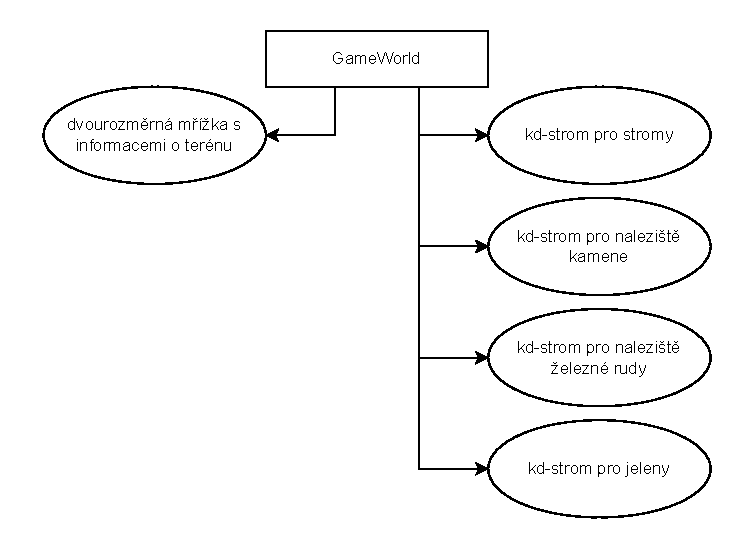
\includegraphics[width=0.8\linewidth]{img/game-world.pdf}
  \caption{Datové struktury obsažené v \texttt{GameWorld}.}
  \label{fig:game-world}
\end{figure}

Instance jednotlivých kd-stromů z obrázku~\ref{fig:game-world} jsou uchovávány v \texttt{Dictionary} uvnitř třídy \texttt{GameWorld}. Toto \texttt{Dictionary} mapuje typ suroviny (instanci třídy \texttt{ResourceType}) na konkrétní kd-strom. Díky tomuto \texttt{Dictionary} můžeme snadno získat kd-strom pro konkrétní typ suroviny.

\subsection{Assety}
Na obrázku~\ref{fig:asset-manager} lze vidět hierarchii tříd souvisejících s managementem assetů. \texttt{AssetManager<TAsset>} obsahuje společnou logiku pro nalezení a načtení assetů ze složky a pro správu slovníku, ve kterém jsou uloženy načtené assety pro generický typ \texttt{TAsset}. Jednotliví potomci této třídy poskytují implementace metody \texttt{Load} pro načtení assetu konkrétního typu. I přesto, že hra momentálně obsahuje pouze assety pro textury a shadery, bylo by díky abstrakci asset managerů snadné hru rozšířit i o jiné typy assetů, jako jsou například zvuky.

\begin{figure}[!htb]
  \centering
  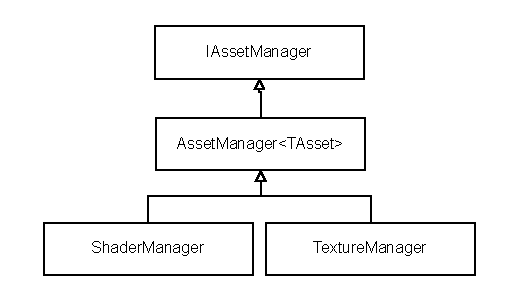
\includegraphics[width=0.6\linewidth]{img/asset-manager.pdf}
  \caption{Hierarchie dědičnosti tříd souvisejících s managementem assetů.}
  \label{fig:asset-manager}
\end{figure}

Všechny assety se nachází ve složce \texttt{Content}. Jednotlivé typy assetů mají poté v této složce svou podsložku. Textury se nacházejí v podsložce \texttt{Textures} a shadery v podsložce \texttt{Shaders}. Je nutné zmínit, že složka \texttt{Shaders} obsahuje již zkompilované shadery.

Veškeré instance rozhraní \texttt{IAssetManager} jsou uchovány ve třídě \texttt{Game}. Pomocí ní je také možné přistupovat k konkrétním instancím (\texttt{ShaderManager} a \texttt{TextureManager}). Při inicializaci hry dojde k zavolání metody \texttt{LoadAll} na každé takové instanci. To vede k načtení všech assetů daného typu.

\subsection{Správa managed typů}
Vytváříme hru, abychom ji později mohli používat pro měření výkonu ECS knihoven. Aby hru pro měření bylo možné použít, je klíčové, aby byla nezávislá na konkrétní ECS knihovně. Z tohoto důvodu hra namísto konkrétní ECS knihovny používá abstrakční vrstvu. V sekci~\ref{sec:components-analysis} jsme si zmínili, že jednotlivé komponenty v abstrakční vrstvě reprezentujeme jako struktury. Ovšem jedna z knihoven, které budeme měřit (konkrétně \textit{Svelto.ECS}~\cite{SveltoECS}), vyžaduje, aby komponenty byly \textit{unmanaged typy}. V této sekci se zaměříme na to, co to jsou \textit{unmanaged typy}, a jak jsme tento problém vyřešili.

Definici \textit{unmanaged typů} lze nalézt ve článku \textit{Unmanaged types (C\# reference)}~\cite{Unmanagedtypes} od firmy \textit{Microsoft}. Ve článku se lze dočíst, že \textit{unmanaged typem} je každý z následujících datových typů:

\begin{enumerate}
  \item \texttt{sbyte}, \texttt{byte}, \texttt{short}, \texttt{ushort}, \texttt{int}, \texttt{uint}, \texttt{long}, \texttt{ulong}, \texttt{nint}, \texttt{nuint}, \texttt{char}, \texttt{float}, \texttt{double}, \texttt{decimal}, nebo \texttt{bool}.

  \item Jakýkoliv výčtový typ.
  
  \item Jakýkoliv typ ukazatele.

  \item Jakýkoliv tuple složený z \textit{unmanaged typů}.

  \item Jakákoliv uživatelem definovaná struktura, která obsahuje pouze fieldy \textit{unmanaged typů}.
\end{enumerate}

Naše komponenty jsou uživatelem definované struktury, tím pádem je pro nás klíčový poslední bod této definice. Konkrétně naše komponenty nesmí obsahovat jiné fieldy, než fieldy \textit{unmanaged typů}. Ovšem v některých případech bychom takové fieldy potřebovali. Jedná se zejména o instance třídy \textit{IEntity} a jakékoliv pole nebo kolekce. Například entity vesničanů v naší hře obsahují \texttt{Villager} komponentu, ve které si uchovávají referenci na entitu vesnice, do které spadají. Dalším příkladem je \textit{PathFollow} komponenta, která přidá entitě schopnost chodit po cestě, která je v této komponentě definována. Cesta je definována za pomocí pole pozic.

Pro řešení tohoto problému byli zavedeny manažery instancí \textit{managed typů}. Na obrázku~\ref{fig:unmanaged-data-managers} lze vidět hierarchii dědičnosti tříd souvisejících s těmito manažery. Prázdný interface \texttt{IManagedDataManager} slouží, abychom mohli instance jednotlivých manažerů spolu ukládat do jedné kolekce. Od tohoto interface dědí abstraktní třída \texttt{ManagedDataManager<TManagedData>}, kde generický parametr \texttt{TManagedData} představuje \textit{managed typ}, jehož instance chceme spravovat. Od této třídy dědí třídy, které se starají o správu konkrétních \textit{managed typů}.

\begin{figure}[!htb]
  \centering
  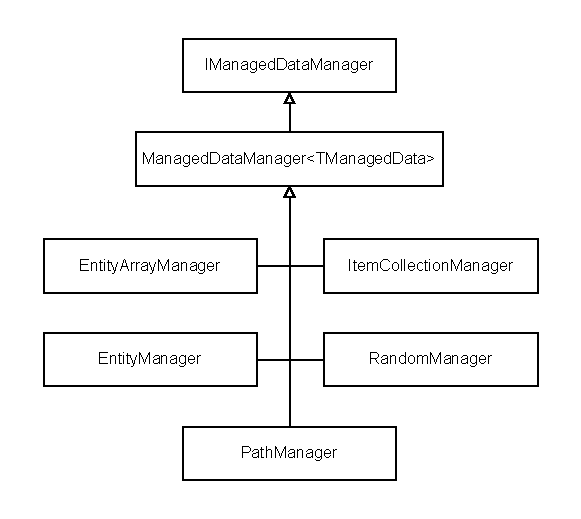
\includegraphics[width=0.6\linewidth]{img/managed_data_managers.pdf}
  \caption{Hierarchie dědičnosti tříd souvisejících se správou instancí \textit{managed typů}.}
  \label{fig:unmanaged-data-managers}
\end{figure}

Třída \texttt{ManagedDataManager<TManagedData>} obsahuje abstraktní metody pro vytváření instancí spravovaného \textit{managed typu}. V jednotlivých manažerech jsou uchovávány spravované instance odpovídajícího \textit{managed typu}. Do manažera je možné instancí vložit nebo vytvořit novou instanci přímo uvnitř manažera. Obě tyto akce nám navrátí ID, za pomoci kterého lze k instancím daného \textit{managed typu} přistupovat. V našich komponentech namísto instancí těchto \textit{managed typů} uchováváme jejich ID.

V případě, že chceme odebrat danou komponentu obsahující ID instance \textit{managed typu}, je nutné odpovídající instanci odebrat z manažera, aby nedošlo k \textit{memory leaku}. V naší hře toto řešíme za pomoci \texttt{DeathSystem}, který řeší smrt entit. V případě smrti entity, tento systém před odstranění dané entity zkontroluje, zda na sobě daná entita nemá komponentu obsahující ID instance \textit{managed typu}. Pokud ano, tak příslušnou instanci odebere z příslušného manažera.

Instance jednotlivých manažerů uchováváme ve třídě \texttt{Game}. Pomocí této třídy je možné k nim také přistupovat. Třídy pro typy jednotlivých manažerů je možné vidět na obrázku~\ref{fig:unmanaged-data-managers}.

\subsection{Uživatelské rozhraní}
Vztahy tříd souvisejících s uživatelským rozhraním je možné vidět na obrázku~\ref{fig:ui-layer}. Třída \texttt{UILayer} je zodpovědná za správu prvků uživatelského rozhraní pro jeden konkrétní herní stav. Každý prvek uživatelského rozhraní dědí od třídy \texttt{UIElement}. Hra momentálně obsahuje pouze jediný prvek uživatelského rozhraní a tím je minimapa (reprezentovaná třídou \texttt{Minimap}), ale je navržena tak, aby bylo snadné ji rozšířit i o další prvky uživatelského rozhraní, jako jsou například labely, tlačítka, nebo action bar.

\begin{figure}[!htb]
  \centering
  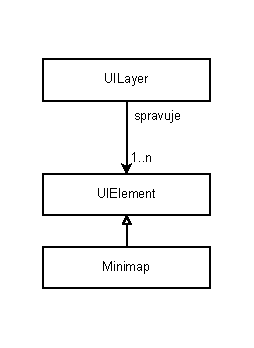
\includegraphics[width=0.35\linewidth]{img/ui-layer.pdf}
  \caption{Diagram vyobrazující vztahy tříd, které souvisejí s uživatelským rozhraním.}
  \label{fig:ui-layer}
\end{figure}

Mezi prvky uživatelského rozhraní existuje stromová hierarchie. Každý prvek může mít několik potomků. Jednotliví potomci poté pracují s pozici relativní vůči svému rodiči.

\subsubsection{Minimapa}
Minimapa je reprezentována třídou \texttt{Minimap}, která dědí od \texttt{UIElement}. Pomocí minimapy chceme znázornit, jak vypadá herní svět a jaká jeho část je momentálně viditelná kamerou. Jejím cílem je usnadnit hráči orientaci v herním světě.

Minimapa se skládá z mapy terénu, view framu a rámečku. Pro vykreslení mapy terénu používáme stejný fragment shader jako pro vykreslení terénu naší hry. Pouze použijeme jiné rozlišení a scale. Poté vykreslíme view frame, ten představuje výsek terénu, který hráč momentálně vidí skrze kameru. Pro jeho vykreslení si najdeme na jakou pozici v minimapě odpovídá umístění kamery a poté vykreslíme obdélníkový rámeček, který odpovídá rozměrům kamery naškálovaných podle velikosti minimapy. Aby nám view frame nepřesahoval hranice minimapy, vykreslujeme jej s nastaveným \texttt{ScissorRectangle}. Jedná se o MonoGame nastavení, pomocí kterého lze provádět oříznutí. Na závěr kolem minimapy vykreslíme rámeček. Ten je reprezentován texturou.

\subsection{Herní data}
Mezi herní data patří informace o biomech, surovinách a předmětech. Herní data jsou immutable a lze k nim přistupovat globálně. Vztahy tříd souvisejících s herními daty je možné vidět na obrázku~\ref{fig:game-data}.

\begin{figure}[!htb]
  \centering
  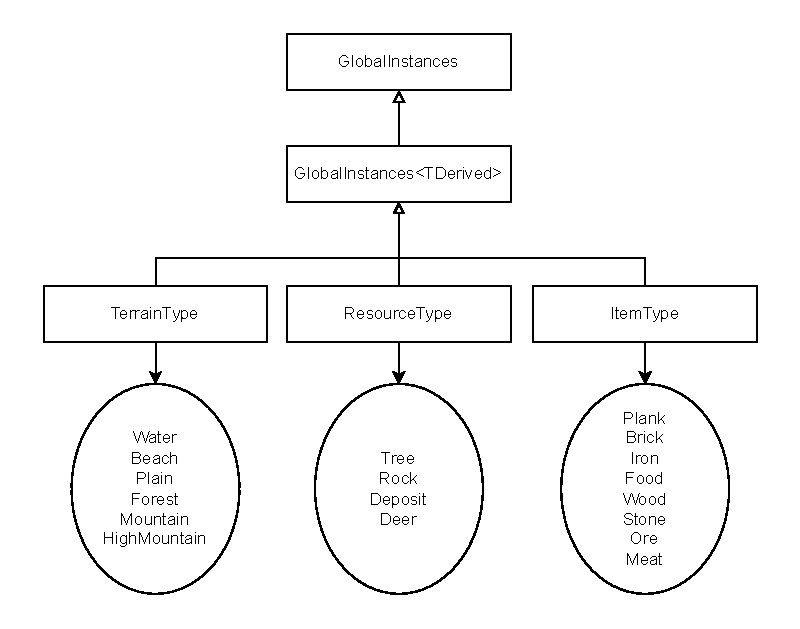
\includegraphics[width=0.7\linewidth]{img/game-data.pdf}
  \caption{Diagram vyobrazující třídy a důležité instance související s herními daty.}
  \label{fig:game-data}
\end{figure}

\texttt{GlobalInstances<TDerived>} je abstraktní třída, kde generický parametr \texttt{TDerived} může být pouze třída, která je jejím potomkem. \texttt{GlobalInstances<TDerived>} si za pomoci statiky interně ukládá všechny instance \texttt{TDerived} a umožňuje k nim globální přístup za pomoci jejich identifikátoru.

Jednotliví potomci třídy \texttt{GlobalInstances<TDerived>} představují jednotlivé typy herních dat, jako je například typ biomu (\texttt{TerrainType}), typ suroviny (\texttt{ResourceType}), nebo typ předmětu (\texttt{ItemType}). Tyto třídy obsahují informace o daném typu herních dat. Například typ biomu (\texttt{TerrainType}) obsahuje informaci o tom, zda je možné v daném biomu stavět, a také informaci o tom, zda je možné v daném biomu chodit.

Je nutné, aby jednotliví potomci třídy \texttt{GlobalInstances<TDerived>} měli privátní konstruktor. Tím zaručíme, že nebude možné vytvářet nové instance mimo danou třídu. Všechny instance těchto potomků jsou definovány jako veřejné readonly statické fieldy přímo uvnitř těchto tříd.  Například herní data reprezentovaná třídou \texttt{TerrainType} obsahují instance pro biom vody (\texttt{Water}), biom pláže (\texttt{Beach}), biom lesa (\texttt{Forest}) a další biomy. Na obrázku~\ref{fig:game-data} lze vidět vypsané jednotlivé instance jednotlivých typů herních dat.

Abstraktní třída \texttt{GlobalInstances} obsahuje pouze module initializer, pomocí kterého zavolá \texttt{RuntimeHelpers.RunClassConstructor} na každém neabstraktním typu, který od ní dědí. Tím máme zaručeno, že naše data jsou v čas vytvořené, jinak by k jejich vytvoření došlo až při prvním přístupu k jejich třídám a do té doby bychom k nim nemohli přistupovat skrze třídu \texttt{GlobalInstances<TDerived>}.

\subsection{Inventáře a předměty}
Na konci sekce~\ref{sec:game-world} jsme si uvedli jednotlivé typy předmětů, které jsou součástí naší hry. Jednotlivé předměty mohou mít vesničané ve svém inventáři (například pokud je získali sklizením suroviny a nyní je odnášejí, aby je zpracovali). Dále jsou předměty skladovány ve skladišti. Vztahy tříd související s předměty je možné vidět na obrázku~\ref{fig:items}.

\begin{figure}[!htb]
  \centering
  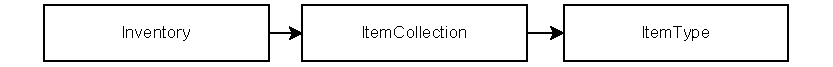
\includegraphics[width=0.8\linewidth]{img/items.pdf}
  \caption{Vztah tříd souvisejících s herními předměty.}
  \label{fig:items}
\end{figure}

Z minulé sekce víme, že instance třídy \texttt{ItemType} reprezentují jednotlivé typy předmětů. Každý typ předmětu má také své ID. Struktura \texttt{ItemCollection} reprezentuje kolekci předmětů. Uvnitř sebe má pole, kde jednotlivé prvky tohoto pole reprezentují počty předmětů uvnitř kolekce. Index každého prvku odpovídá ID daného typu předmětu. Například předmět \textit{prkno} má ID 0 a element z tohoto pole s indexem 0 odpovídá počtu prken uvnitř dané kolekce. Kromě tohoto pole struktura \texttt{ItemCollection} také obsahuje pomocné metody pro manipulaci s kolekcemi předmětů.

Třída \texttt{Inventory} je komponenta. Entity s touto komponentou mají inventář, do kterého mohou ukládat předměty. Tato třída obsahuje jediný field a tím je ID na instanci \texttt{ItemCollection}. Tuto komponentu na sobě kromě entit vesničanů a skladišť mají také entity budov pro zpracování předmětů (například budova dřevorubce). Do tohoto inventáře přesouvají vesničané předměty pro zpracování, a entita dané budovy pro zpracování surovin zde také ukládá produkt získaný zpracováním daného předmětu.

\subsection{Suroviny}
\label{sec:res-impl}
Jednotlivé suroviny jsou reprezentovány jako entity. Komponenty, ze kterých jsou tyto entity složené, a systémy, které tyto komponenty zpracovávají, je možné vidět na obrázku~\ref{fig:resource}. \texttt{RenderSystem} se stará o vykreslení entity. \texttt{Appearance} komponenta nese informaci o tom, jak entita vypadá, a \texttt{Location} obsahuje informaci o tom kde se nachází. \texttt{DeathSystem} řeší logiku smrti dané entity, konkrétně v případě surovin dojde k jejich smrti v případě sklizení.

\begin{figure}[!htb]
  \centering
  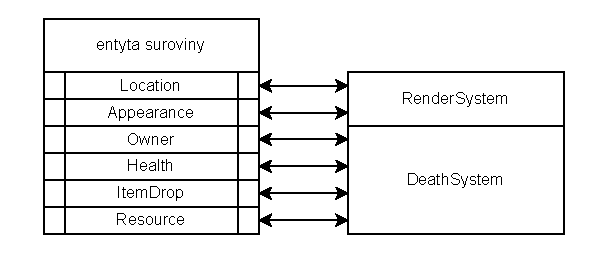
\includegraphics[width=0.8\linewidth]{img/resource.pdf}
  \caption{Entita suroviny s jejími komponentami a systémy, které tyto komponenty zpracovávají.}
  \label{fig:resource}
\end{figure}

Každá surovina má \texttt{Health} komponentu, ve které je uložena informace o aktuálním počtu životů. Entita obsahující \texttt{DamageDealer} komponentu může zaútočit na entitu obsahující \texttt{Health} komponentu. Při tomto útoku se počet životů v příslušné \texttt{Health} komponentě sníží a pokud klesne na nulu, tak \texttt{DeathSystem} kromě smazání mrtvé entity nahlédne, zda zemřelá entita obsahuje \texttt{ItemDrop} komponentu. Pokud ano, tak předměty definované v této komponentě převede do inventáře entity, která danou entitu zabila. Stejným způsobem funguje i sklízení surovin, kde útočící entitou je vesničan, který útočí na entitu dané suroviny a tím ji sklízí. Po jejím zabití neboli sklizení obdrží do svého inventáře příslušné předměty.

Suroviny na sobě mají také \texttt{Owner} komponentu. Ta obsahuje instanci typu dědícího od \texttt{IEntity}, která reprezentuje danou entitu. \texttt{DeathSystem} vyžaduje tuto komponentu, aby mohl danou entitu smazat.

Jak již bylo zmíněno, existuje kd-strom pro každý typ suroviny. Jedná se o datovou strukturu, pomocí které lze efektivně vyhledávat v prostoru. Entity jednotlivých surovin jsou uloženy v těchto kd-stromech. Tyto kd-stromy poté využívají vesničané, kteří v rámci svého povolání provádějí úlohu nalezení nejbližší suroviny daného typu. Pokud si vesničan rezervuje danou surovinu (začne pohyb směrem k ní a následně ji sklidí), dojde k odebrání této suroviny z příslušného kd-stromu. Tím zamezíme tomu, že více vesničanů nebude sklízet stejnou entitu suroviny. Pro implementaci kd-stromu používáme Nugget balíček \textit{KdTree}~\cite{KdTree}.

Dále je nutné zmínit, že \texttt{DeathSystem} pracuje nad všemi entitami s komponentami \texttt{Health} a \texttt{Owner}. V případě, že zemřelá entita má na sobě komponentu \texttt{Inventory} nebo komponentu \texttt{ItemDrop}, tak převede dané předměty. A v případě, že zemřelá entita je vesničan a ten útočil na entitu s komponentou \texttt{Resource} (daná entita byla surovina), tak je nutné entitu vrátit do příslušného kd-stromu.

Entita \textit{jelena} se od ostatních entit surovin liší. Její komponenty a systémy, které zpracovávají tyto komponenty, je možné vidět na obrázku \ref{fig:deer}. Je možné nahlédnout, že oproti entitám ostatních surovin má entita \textit{jelena} navíc komponenty \texttt{Movement}, která přidává entitám schopnost chodit a \texttt{AnimalBehavior}. \texttt{AnimalBehaviorSystem} poté pracuje se všemi entitami s komponentami \texttt{Location}, \texttt{Owner}, \texttt{Movement} a \texttt{AnimalBehavior} a jeho hlavním úkolem je řídit chování zvířat, konkrétně jejich náhodný pohyb. Krom tohoto úkolu se tento systém stará také o aktulizaci pozice entit zvířat v příslušném kd-tree.

\begin{figure}[!htb]
  \centering
  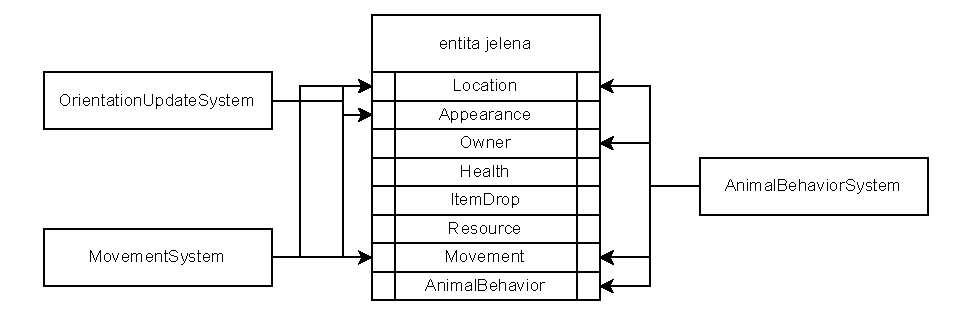
\includegraphics[width=1.0\linewidth]{img/deer.pdf}
  \caption{Entita jelena s jejími komponentami a systemy \texttt{AnimalBehaviorSystem}, \texttt{MovementSystem} a \texttt{OrientationUpdateSystem}.}
  \label{fig:deer}
\end{figure}

\texttt{MovementSystem} se stará o pohyb entit. Jak \texttt{MovementSystem}, tak \texttt{AnimalBehaviorSystem}, pracují s \texttt{Movement} komponentou, ale \texttt{AnimalBehaviorSystem} řídí, jak se pohyb bude odehrávat a \texttt{MovementSystem} se stará o samotný pohyb. \texttt{OrientationUpdateSystem} aktualizuje orientaci entity. V závislosti na tom, zda se entita pohybuje doleva nebo doprava, tak převrátí texturu dané entity podle osy y, aby její orientace odpovídala směru, ve kterém se pohybuje.

\subsection{Vesnice a vesničané}
Ze sekce~\ref{subsec:villages} víme, že v herním světě se budou nacházet vesničané a vesnice. Jednotlivé vesnice budou obsahovat budovy. Každá budova, každý vesničan a i samotná vesnice jsou reprezentovány jako entity. V této sekci si tyto entity představíme.

\subsubsection{Vesničané}
Diagram s entitou vesničana je možné vidět na obrázku~\ref{fig:villager}. Kromě vyobrazených systémů souvisí s vesničanem také \texttt{MovementSystem}, \texttt{DeathSystem}, \texttt{OrientationUpdateSystem} a \texttt{RenderSystem}. Tyto systémy byly popsány v minulé sekci a nyní se jim nebudeme věnovat.

\begin{figure}[!htb]
  \centering
  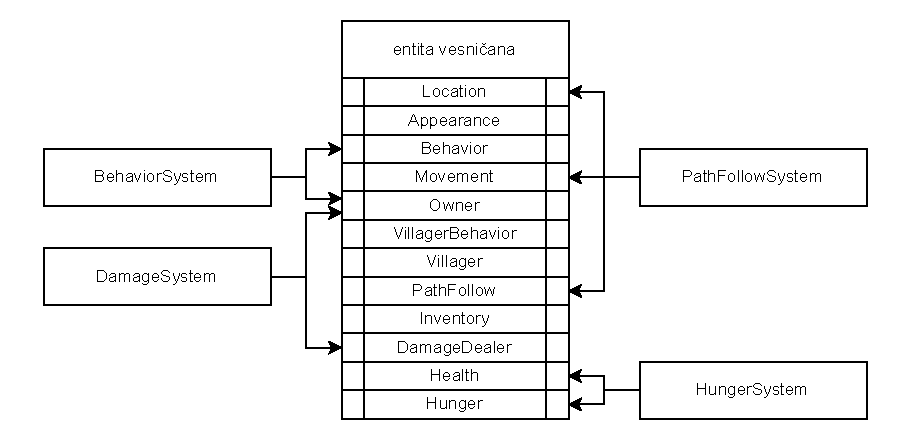
\includegraphics[width=1.0\linewidth]{img/villager.pdf}
  \caption{Entita vesničana s jejími komponentami a systemy \texttt{BehaviorSystem}, \texttt{PathFollowSystem}, \texttt{DamageSystem} a \texttt{HungerSystem}.}
  \label{fig:villager}
\end{figure}

Již zmiňovaný \texttt{DamageSystem} řeší logiku poškození. Z minulé sekce víme, že díky tomuto systému je vesničanům umožněno sklízet suroviny. \texttt{HungerSystem} řeší logiku hladovění. V \texttt{Hunger} komponentě je uložen aktuální stav hladovění vesničana. Tento stav neustále roste a pokud přesáhne určitou hranici, vesničan začne ztrácet životy. Pokud vesničan sní jídlo, stav hladovění se nastaví na nulu.

\texttt{BehaviorSystem} se stará o chování vesničanů. Ze sekce~\ref{sec:ai} víme, že pro chování vesničanů používáme \textit{strom chování}. Každý vesničan má právě jeden \textit{strom chování} a \texttt{BehaviorSystem} pouze volá metodu \textit{Tick} na daném \textit{stromě chování}, která jej zpracovává.

Některé části z tohoto \textit{BehaviorTree} každého vesničana se starají o generování cest. Například pokud vesničan potřebuje dojít k entitě dané suroviny. Vygenerovaná cesta je poté uložena do \texttt{PathFollow} komponenty. O logiku chození po cestě se stará \texttt{PathFollowSystem}. Je nutné zmínit, že samotný pohyb vždy řeší \texttt{MovementSystem}, \texttt{PathFollowSystem} pouze nastavuje hodnoty v \texttt{Movement} komponentě na základě cesty uložené v \texttt{PathFollow} komponentě.

\subsubsection{Budovy}
Diagram entity budovy je možné vidět na obrázku~\ref{fig:building}. Vyobrazené komponenty má na sobě každá budova. V komponentě \texttt{Village} je uchováván odkaz na instanci vesnice, do které budova spadá. Budova skladiště má na sobě navíc \texttt{Inventory} komponentu, ve které ukládá suroviny, které vesnice vlastní. Hlavní budova, oproti diagramu, neobsahuje žádné dodatečné komponenty.

\begin{figure}[!htb]
  \centering
  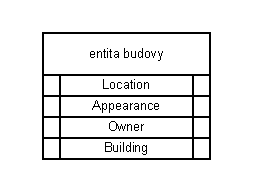
\includegraphics[width=0.4\linewidth]{img/building.pdf}
  \caption{Entita budovy s jejími komponentami.}
  \label{fig:building}
\end{figure}

Důležitým typem budov jsou budovy pro zpracování surovin. Diagram vyobrazující jejich komponenty a související systémy je možné vidět na obrázku~\ref{fig:res_building}. Je možné vidět, že oproti entitě z obrázku~\ref{fig:building} má budova pro zpracování surovin navíc komponenty \texttt{Inventory}, \texttt{ResourceProcessor} a \texttt{VillagerSpawner}.

\begin{figure}[!htb]
  \centering
  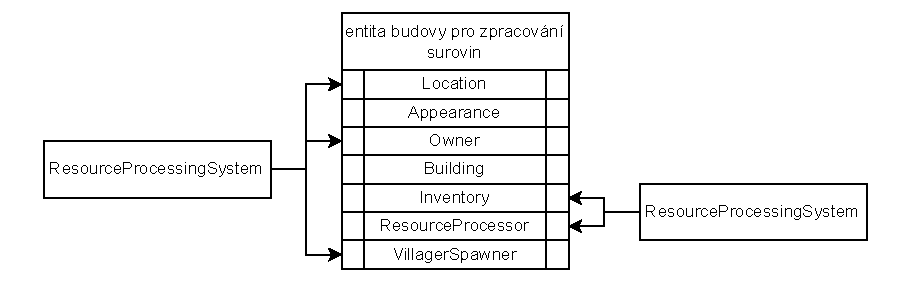
\includegraphics[width=1.0\linewidth]{img/resource_building.pdf}
  \caption{Entita budovy pro zpracování surovin s jejími komponentami a systémy \texttt{ResourceProcessingSystem} a \texttt{VillagerSpawningSystem}.}
  \label{fig:res_building}
\end{figure}

\texttt{VillagerSpawningSystem} je zodpovědný za vytváření nových vesničanů. Ke každé budově pro zpracování surovin je přidělen právě jeden vesničan, a pokud tento vesničan zemře, tak se spustí odpočet. Po uplynutí tohoto odpočtu dojde k vytvoření nového vesničana. Při jeho vytvoření mu bude zkonstruován a přidělen \textit{strom chování} a příslušná budova mu bude nastavena jako pracovní místo.

\texttt{ResourceProcessingSystem} se stará o logiku kolem zpracování surovin. Budovy pro zpracování surovin na sobě mají \texttt{Inventory} komponentu. \texttt{ResourceProcessingSystem} má na sobě nastavený recept a pravidelně nahlíží, zda se v inventáři dané suroviny nacházejí požadované suroviny. Pokud ano, tak zahájí zpracování, po jehož dokončení přemístí nově vytvořené předměty opět do inventáře. Z něj je může vesničan převzít a odnést do skladiště.

\subsubsection{Vesnice}
Každá vesnice je entita, která obsahuje komponenty \texttt{Location}, \texttt{Village} a \texttt{Owner}. \texttt{VillageBuildingSystem} se stará o stavění budov v dané vesnici. Má v sobě uloženou stavební frontu budov, kde pro každou budovu má také její cenu. Ve \texttt{Village} komponentě jsou uchovávány odkazy na jednotlivé entity budov, které se ve vesnici nacházejí. Jakmile \texttt{VillageBuildingSystem} zjistí, že vesnice má dostatek surovin na další budovu ze stavební fronty, vytvoří pro ni entitu a přidá na vytvořenou entitu odkaz do \texttt{Village} komponenty.

Klíčovou částí při vytváření entity budovy je volba pozice, kde se entita má vytvořit. Nechceme, aby budovy byly umístěny v biomech, kde nelze stavět, a také nechceme, aby se nacházely moc blízko nebo moc daleko od ostatních budov. Pro volbu pozice budov je zvolena konstantní minimální a maximální vzdálenost. Tyto vzdálenosti udávají, v jakém rozmezí se mohou nové budovy od již postavených budov objevit.

Pro volbu pozice byl použit přímočarý algoritmus. Jako první se vybere náhodná již postavená budova a vezme se její pozice. Poté se kolem této pozice vytvoří prstenec s rozměry podle konstantní minimální a maximální vzdálenosti. V tomto prstenci se poté vybere náhodná pozice. Na závěr se zkontroluje, zda je možné na této pozici stavět, a pokud ano, tak je tato pozice vybrána jako pozice pro novou budovu. Pokud na dané pozici není možné stavět, tak se celý algoritmus zopakuje.

\section{Měření}
\label{benchmark-implementation}
Měření je druhým C\# projektem (\texttt{WorldSimulator.Benchmarks.csproj}) našeho C\# solution. S použitím naší hry měří výkon jednotlivých ECS knihoven. V sekci~\ref{benchmark-framework} jsme se rozhodli, že pro toto měření použijeme \textit{BenchmarkDotNet}. Celé měření se dělí na dvě fáze, a to přípravy a samotného měření.

Pro měření máme definované následující konstanty:

\begin{enumerate}
  \item \texttt{seed}: Seed pro generování náhodných čísel. Stejným seedem pro každé měření zajistíme konzistentnost.

  \item \texttt{deltaTime}: Čas v sekundách. Tento čas používáme pro odsimulovaní jednoho kroku naší hry (jedné iterace \textit{game loop}, který byl přiblížen v sekci~\ref{game-loop}).

  \item \texttt{setupIterationCount} Udává počet kroků odsimulování naší hry během fáze přípravy.

  \item \texttt{benchmarkIterationCount}: Udává počet kroků odsimulování hry během fáze měření.
\end{enumerate}

V C\# projektu (\texttt{WorldSimulator.Benchmarks.csproj}) máme definovaný test reprezentovaný třídou \texttt{ECSBenchmarks}. Tento test obsahuje jediný vstupní parametr, a tím je \texttt{ECSFactoryType} typu \texttt{Type}. Tímto parametrem jsou předávány typy dědící od \texttt{ECSFactory}, které reprezentují jednotlivé ECS knihovny.

Během fáze přípravy nejprve zkonstruujeme konkrétní \texttt{ECSFactory}. Poté vytvoříme novou instanci naší hry (třídy \texttt{Game}) a odsimulujeme jeden její snímek za pomocí \texttt{RunOneFrame}, tím zaručíme, že hra bude inicializována. Poté v cyklu voláme metodu \texttt{UpdateOnce}, která vykoná jednu iteraci \textit{game loop} naší hry. Počet opakování tohoto cyklu udává konstanta \texttt{setupIterationCount}.

Během fáze měření používáme tu samou instanci hry vytvořenou během fáze přípravy. Na této instanci v cyklu opět zavoláme metodu \texttt{UpdateOnce}. Počet opakování tohoto cyklu je dán konstantou \texttt{benchmarkIterationCount}.

% \newpage
% \null










% \subsection{Herní mechaniky}
% Implementace jednotlivých herních mechanik je možné najít v jednotlivých systémech (myšleno typech dědicích od \texttt{IEntityProcesor}) a komponentách. Všechny komponenty se nacházejí ve jmenném prostoru \texttt{WorldSimulator.Components}. Všechny systémy v \texttt{WorldSimulator.Systems}.

% Některé systémy se zabývají vykreslováním hry. Tyto systémy se reprezentují stejným způsobem jako běžné systémy, akorát k jejich vytvoření dojde v metodě \texttt{GameState.CreateRenderSystems} namísto metody \texttt{GameState.CreateSystems}, ve které se běžně vytvářejí systémy.




















% \begin{enumerate}
%     \item \textbf{\texttt{IECSSystem}:} Jedná se o rozhraní. Instance typů, které implementují toto rozhraní, představují kompletní systém. Tyto typy obsahují logiku pro iteraci přes jednotlivé entity. O zpracování jednotlivých entit se stará \texttt{EntityProcessor}. Každá instance kompletního systému má na sobě právě jeden \texttt{EntityProcessor}. Například \texttt{ArchSystem<TEntityProcessor, TComponent>} je systém, který obsahuje logiku pro procházení entit z ECS knihovny \textit{Arch}~\cite{Arch}.

%     \item \textbf{\texttt{IEntityProcesor}:} Jedná se o rozhraní, které ma na sobě klíčovou metodu \texttt{Process}. Typy, které implementují toto rozhraní obsahují herní logiku, která zpracovává jednotlivé entity. Například \verb|MovementSystem| ve své metodě \verb|Process| zpracuje pohyb pro danou entitu.

%     Z pohledu hry jednotlivé implementace \textit{EntityProcessor} představují samotné systémy, jelikož hra nekouká na to jak jsou entity iterovány a zajímá je jenom samotná herní logika. Proto se kód, který pracuje s hrou odkazuje na \texttt{EntityProcessor} jako na systém. Ovšem z pohledu abstrakční vrstvy je nutné rozlišovat \texttt{System} jako typ, který obsahuje logiku pro iteraci entit a \texttt{EntityProcessor} jako typ, který obsahuje logiku pro zpracování entit. Autor si je vědom, že tyto pohledy mohou vést k matoucí terminologii, ovšem v kódu jsou již používány na příliš mnoho místech.

%     \item \textbf{\texttt{}:} Jedná se o rozhraní. Typy, které implementují toto rozhraní definují logiku pro vytváření entity a \textit{world} dané implementace abstrakční vrstvy. Pomocí instancí těchto typů je také možné vytvářet instance kompletních systémů. Tyto typy také reprezentují celou jednu implementaci abstrakční vrstvy.

%     \item \textbf{\texttt{IECSWorld}:} Jedná se rozhraní. Typy, které implementují toto rozhraní, představují \textit{world} pro danou ECS knihovnu. Jelikož pro velkou část ECS knihoven typy, které implementovali toto rozhraní, vypadali identicky, byl zaveden typ \texttt{BasicECSWorld}. Tento typ lze použít pro většinu ECS knihoven.

%     \item \textbf{\texttt{IEntity}:} Jedná se o rozhraní. Typy, které implementují toto rozhraní představují entitu v konkrétní ECS knihovně.

%     \item \textbf{\texttt{ComponentAttribute}:}. Některé ECS knihovny potřebují před spuštěním hry vědět o typech všech komponent, které budou ve hře používány. Proto je typ jakékoliv komponenty označen tímto atributem a v případě, že některá ECS knihovna bude potřebovat znát typy jednotlivých komponent, může si skrze reflexi najít všechny typy s tímto atributem.
% \end{enumerate}






% Popis a provázanost členů. Co musí ECS knihovna implementovat. V jakém je to namespace.

% \section{Hra}

% Popis a provázanost  členů.

% \subsection{Herní svět}












% V této kapitole si představíme klíčové a zajímavé části implementace naší hry. Pro více detailů o implementaci je možné nahlédnout do kódu, který obsahuje dokumentační komentáře.

% Pro tvorbu hry byl použit MonoGame framework~\cite{MonoGame}, ovšem základní MonoGame nemá podporu pro compute shadery, které jsme využili pro řešení problému s vyhledávání cesty v podsekci~\ref{subsection:path-finding}. Z toho důvodu byl použit fork~\cite{MonoGameCptMax}, který tuto podporu nabízí.

% \section{Abstrakční vrstva}
% \label{sec:abstract-layer}
% Některé typy z abstrakční vrstvy jsme si již představili v sekci \ref{section:abstract-layer-analysis}. Pro připomenutí si nyní tyto typy lehce představíme znovu a zároveň si popíšeme další důležité typy z abstrakční vrstvy:

% \begin{enumerate}
%     \item \textbf{\texttt{IECSSystem}:} Jedná se o rozhraní. Instance typů, které implementují toto rozhraní, představují kompletní systém. Tyto typy obsahují logiku pro iteraci přes jednotlivé entity. O zpracování jednotlivých entit se stará \texttt{EntityProcessor}. Každá instance kompletního systému má na sobě právě jeden \texttt{EntityProcessor}. Například \texttt{ArchSystem<TEntityProcessor, TComponent>} je systém, který obsahuje logiku pro procházení entit z ECS knihovny \textit{Arch}~\cite{Arch}.

%     \item \textbf{\texttt{IEntityProcesor}:} Jedná se o rozhraní, které ma na sobě klíčovou metodu \texttt{Process}. Typy, které implementují toto rozhraní obsahují herní logiku, která zpracovává jednotlivé entity. Například \verb|MovementSystem| ve své metodě \verb|Process| zpracuje pohyb pro danou entitu.

%     Z pohledu hry jednotlivé implementace \textit{EntityProcessor} představují samotné systémy, jelikož hra nekouká na to jak jsou entity iterovány a zajímá je jenom samotná herní logika. Proto se kód, který pracuje s hrou odkazuje na \texttt{EntityProcessor} jako na systém. Ovšem z pohledu abstrakční vrstvy je nutné rozlišovat \texttt{System} jako typ, který obsahuje logiku pro iteraci entit a \texttt{EntityProcessor} jako typ, který obsahuje logiku pro zpracování entit. Autor si je vědom, že tyto pohledy mohou vést k matoucí terminologii, ovšem v kódu jsou již používány na příliš mnoho místech.

%     \item \textbf{\texttt{}:} Jedná se o rozhraní. Typy, které implementují toto rozhraní definují logiku pro vytváření entity a \textit{world} dané implementace abstrakční vrstvy. Pomocí instancí těchto typů je také možné vytvářet instance kompletních systémů. Tyto typy také reprezentují celou jednu implementaci abstrakční vrstvy.

%     \item \textbf{\texttt{IECSWorld}:} Jedná se rozhraní. Typy, které implementují toto rozhraní, představují \textit{world} pro danou ECS knihovnu. Jelikož pro velkou část ECS knihoven typy, které implementovali toto rozhraní, vypadali identicky, byl zaveden typ \texttt{BasicECSWorld}. Tento typ lze použít pro většinu ECS knihoven.

%     \item \textbf{\texttt{IEntity}:} Jedná se o rozhraní. Typy, které implementují toto rozhraní představují entitu v konkrétní ECS knihovně.

%     \item \textbf{\texttt{ComponentAttribute}:}. Některé ECS knihovny potřebují před spuštěním hry vědět o typech všech komponent, které budou ve hře používány. Proto je typ jakékoliv komponenty označen tímto atributem a v případě, že některá ECS knihovna bude potřebovat znát typy jednotlivých komponent, může si skrze reflexi najít všechny typy s tímto atributem.
% \end{enumerate}

% \section{Páteřní kód}
% Páteřní kód naší hry se skládá z následujících tříd:

% \begin{enumerate}
%     \item \textbf{\texttt{Game}:} Tato třída představuje samotnou hru. Dědí od třídy \texttt{Microsoft.Xna} \texttt{.Framework.Game} a přetěžuje od ní klíčové metody \verb|Update| a \verb|Draw|. Tato třída přijímá skrze konstruktor instanci typu, který implementuje rozhraní \texttt{}. Pomocí této instance je možné zvolit konkrétní implementaci abstrakční vrstvy neboli konkrétní ECS knihovnu se kterou bude hra pracovat.

%     \item \textbf{\texttt{GameState}:} Abstraktní třída \verb|GameState| představuje herní obrazovku. Herní obrazovky mohou být například Menu, Nastavení, nebo Level. I přesto, že naše hra obsahuje pouze jednu herní obrazovku, díky této třídě by bylo jednoduché do hry výše zmíněné herní obrazovky přidat.

%     \verb|GameState| si v sobě uchovává všechny systémy, které jsou rozděleny do dvou kolekcí. První je kolekce \verb|renderSystems|, která obsahuje všechny systémy, které řeší vykreslování. Druhá kolekce je \verb|systems|, která obsahuje všechny ostatní systémy.

%     \verb|GameState| má na sobě definované dvě klíčové metody a to \verb|Update| a \verb|Draw|. V \verb|Update| se zpracují všechny systémy z kolekce \verb|systems| a v \verb|Draw| se zpracují všechny systémy z kolekce \verb|renderSystems|.

%     \texttt{Game} má v jeden moment aktivní pouze jedenu herní obrazovku pro kterou ve své metodě \texttt{Update} volá \texttt{Update} na této herní obrazovce a ve své metodě \texttt{Draw} volá \texttt{Draw} na této herní obrazovce.

%     Mezi důležité členy, které \verb|GameState| obsahuje patří:

%     \begin{enumerate}
%         \item \textbf{\texttt{ECSWorld}:} Tento člen implementuje rozhraní \verb|IECSWorld| a představuje správce všech entit a komponent uvnitř jednoho \verb|GameState|.
%         \item \textbf{\texttt{Camera}:} Představuje herní kameru.
%         \item \textbf{\texttt{UILayer}:} Jedná se o správce prvků uživatelského rozhraní uvnitř jednoho \verb|GameState|.
%     \end{enumerate}

%     \verb|GameState| obsahuje metodu \verb|Initialize| ve které jsou volány abstraktní metody \verb|CreateEntities|, \verb|CreateSystems|, \verb|CreateRenderSystems| a \verb|CreateUI|, pomocí kterých jednotlivý potomci vytvářejí své entity, systémy a prvky uživatelského rozhraní.

%     \item \textbf{\texttt{LevelState}:} Třída \verb|LevelState| dědí od třídy \verb|GameState| a reprezentuje herní obrazovku, která obsahuje samotný level.

%     \item \textbf{\texttt{LevelFactory}:} Třída \verb|LevelFactory| obsahuje metody pro vytváření jednotlivých entit, která jsou používané v \verb|LevelState|.
% \end{enumerate}

% \section{Herní svět}
% Herní svět je reprezentován třídou \verb|GameWorld|. Tato třída obsahuje grid s informacemi o terénu, který je použit pro hledání cest. Do herního světa je možné přidávat suroviny skrze metodu \verb|AddResource|. Je také možné se dotazovat na informace ohledně terénu na konkrétní pozici v herním světě skrze metody \verb|GetTerrain|, \verb|CanWalkAt|, \verb|CanBuildAt|.

% O generování herního světa se stará třída \verb|GameWorldGenerator|. Při generování světa se nejprve vygeneruje samotný terén, poté dojde ke generování surovin a následně ke generování vesnic.

% Pro generování světa používáme dva shadery, konkrétně fragment shader pro vykreslování terénu, definovaný v souboru \textit{terrainDraw.fx} a compute shader pro generování dvourozměrného pole, které se používá pro hledání cest, definovaný v souboru \textit{terrainGen.fx}. Oba shadery využívají společnou část definovanou v souboru \textit{terrain.fx}.

% Společná část definovaná v souboru \textit{terrain.fx} je zodpovědná za generování terénu. Pro generování terénu je použit simplexův šum na jehož generování je využita knihovna lygia~\cite{lygia}. Pomocí simplexova šumu je vygenerována výšková mapa, která je poté namapována v příslušné biomy. Ve společné části jsou definované dvě důležité funkce a to \verb|CalcNoise|, která spočítá výšku pro specifikovanou pozici a \verb|GetTerrain|, která přijme výšku a na základě ní navrátí informace o daném biomu, který je pro tuto výšku mapován.

% Compute shader definovaný v souboru \textit{terrainGen.fx} přijímá jako vstupní parametry velikost herního světa a vzdálenost mezi jednotlivými body, které budou samplovány do již zmiňovaného 2D pole (viz sekce \ref{subsection:path-finding}). Mezi výstupy patří dva důležité buffery. Prvním je \verb|terrainBuffer|, který pro každý bod v gridu obsahuje identifikátor příslušného terénu. Druhým je \verb|resourceBuffer|, který obsahuje pozice na kterých bude vygenerována surovina.

% Fragment shader definovaný v souboru \textit{terrainDraw.fx} je zodpovědný za vykreslení oblasti z herního světa. Mezi jeho vstupní parametry patří velikost světa, velikost okna, přiblížení kamery a pozice kamery. Tento shader je použit kromě vykreslování samotného herního světa také k vykreslení minimapy.

% O samotné vykreslování herního světa se stará \texttt{TerrainRenderSystem}, který pro vykreslení volá fragment shader definovaný v souboru \textit{terrainDraw.fx}.

% \section{Herní data a jejich reprezentace}
% Pro reprezentaci některých dat v naší hře, může být užitečné mít zavedené datové typy, pro které budeme mít globální přístup ke každé instanci těchto typů. Mezi tyto data mohou patřit například suroviny (třída \texttt{ResourceType}), předměty (třída \texttt{ItemType}), nebo biomy (třída \texttt{TerrainType}).

% Pro reprezentaci těchto dat je zavedena třída \texttt{GlobalInstances}, která jako generický argument \texttt{TDerived} přijímá typ, který od této třídy dědí. Tato třída má interní statickou kolekci, ve které jsou uloženy všechny vytvořené instance třídy \texttt{TDerived}. Třída \texttt{GlobalInstances} je také zodpovědná za generování číselného identifikátoru pro každou instanci \texttt{TDerived}. Tento identifikátor slouží zároveň jako index dané instance. Konkrétní instanci lze získat skrze metodu \texttt{Get}, která navrátí instanci podle specifikovaného indexu.

% Jednotlivé typy, které dědí od \texttt{GlobalInstances} mají privátní konstruktor a všechny své instance definují přímo v sobě jako veřejné readonly statické členy.

% Následující kód je definicí surovin z naší hry a slouží jako příklad použití \texttt{GlobalInstances}:

% \begin{verbatim}
% /// <summary>
% /// Represent a type of a natural resource, which can
% /// be harvested to obtain items.
% /// </summary>
% internal sealed class ResourceType
%   : GlobalInstances<ResourceType>
% {
%   /// <summary>
%   /// The item obtained upon harvesting the resource.
%   /// </summary>
%   public ItemType HarvestItem { get; init; }
%   /// <summary>
%   /// The number of items obtained upon harvesting
%   /// the resource.
%   /// </summary>
%   public int HarvestQuantity { get; init; }
%   /// <summary>
%   /// How much time it takes to harvest the resource
%   /// in seconds.
%   /// </summary>
%   public float HarvestTime { get; init; }
%   private ResourceType() : base() { }
%   public readonly static ResourceType Tree = new()
%   {
%     HarvestItem = ItemType.Wood,
%     HarvestQuantity = 1,
%     HarvestTime = 3.0f,
%   };
%   public readonly static ResourceType Rock = new()
%   {
%     HarvestItem = ItemType.Stone,
%     HarvestQuantity = 1,
%     HarvestTime = 5.0f,
%   };
%   public readonly static ResourceType Deposit = new()
%   {
%     HarvestItem = ItemType.Ore,
%     HarvestQuantity = 1,
%     HarvestTime = 7.0f,
%   };
%   public readonly static ResourceType Deer = new()
%   {
%     HarvestItem = ItemType.Meat,
%     HarvestQuantity = 1,
%     HarvestTime = 9.0f,
%   };
% }
% \end{verbatim}

% \section{Herní mechaniky}
% Implementace jednotlivých herních mechanik je možné najít v jednotlivých systémech (myšleno typech dědicích od \texttt{IEntityProcesor}) a komponentách. Všechny komponenty se nacházejí ve jmenném prostoru \texttt{WorldSimulator.Components}. Všechny systémy v \texttt{WorldSimulator.Systems}.

% Některé systémy se zabývají vykreslováním hry. Tyto systémy se reprezentují stejným způsobem jako běžné systémy, akorát k jejich vytvoření dojde v metodě \texttt{GameState.CreateRenderSystems} namísto metody \texttt{GameState.CreateSystems}, ve které se běžně vytvářejí systémy. Za implementaci obou těchto metod jsou zodpovědní potomci třídy \texttt{GameSystem}.

% \section{Vesnice a vesničané}
% Jednotlivé vesnice jsou reprezentovány jako entity. Tyto entity na sobě mají \texttt{Village} komponentu, ve které si uchovávají seznam svých budov.

% Budovy jsou také reprezentovány jako entity. Entity budov na sobě mají \texttt{Building} komponentu, ve které si uchovávají entitu vesnice, do které spadají.

% Budovy pro zpracování surovin na sobě navíc mají \texttt{ResourceProcessor} komponentu. Tyto budovy se starají o zpracování surovin podle daného receptu, který mají uložen v této komponentě. Mechaniku pro zpracování surovin řeší \texttt{ResourceProcessingSystem}.

% Budovy pro zpracování surovin mají na sobě také \texttt{VillagerSpawner} komponentu. Ta je společně s \texttt{VillagerSpawningSystem} zodpovědná za mechaniku  vesničanů. Tato komponenta v sobě uchovává informace o tom jak dlouho trvá než dojde ke spawnutí vesničana a o profesi, která bude spawnutému vesničanovi přidělena. V případě, že vesničan zemře, začne odpočet a po jeho ukončení dojde ke spawnutí nového vesničana.

% village building system

% villagers

% \xxx{TODO}





























% \chapter{Popis implementace}
% V této kapitole si blíže představíme implementaci naší hry.

% \section{Abstrakce}
% Prvně si rozebereme jak vypadá páteřní kód naší hry.

% % Game, GameState, LevelState, Factory, LevelFactory

% Nyní si přibližme naší abstrakční vrstvu Abstract.ECS.

% % \xxx{Code base}
% % \\
% % \xxx{Abstract.ECS layer}

% \section{Herní svět}
% Herní svět je reprezentován třídou GameWorld.

% O generování herního světa se stará třída GameWorldGenerator.

% Rozeberme si co jsou to vlastně shadery.

% Naše hra používá dva shadery.

% % \xxx{GameWorld}
% % \\
% % \xxx{GameWorldGenerator}
% % \\
% % \xxx{Shaders}

% \section{Herní data a jejich reprezentace}

% Pro správu herních dat, slouží třída GlobalInstances.

% % co jsou herni data, co trida dela

% % \xxx{Data - biomes, items, and resources}

% \section{Systémy a komponenty}

% Následující seznam obsahuje a popisuje všechny herní systémy a komponenty.
\include{5_benchmark}
\chapter{Závěr}
V této kapitole zhodnotíme zda jsme splnili cíle práce. Nejprve se zaměříme na splněné cíle a uvedeme si nedostatky našeho řešení. Na závěr nahlédneme na možná budoucí vylepšení.

\section{Cíle}
Nyní si připomeňme jaké jsou cíle této práce:

\begin{enumerate}
    \item[1)] Vytvořit hru pomocí ECS, která bude nezávislá na konkrétní ECS knihovně.
    \item[2)] Pomocí vytvořené hry porovnat relativní výkon populárních ECS knihoven pro programovací jazyk C\#.
\end{enumerate}

\subsection{Splnění cíle 1}
Pro splnění cíle 1 byla vytvořena hra. Specifikaci této hry jsme stanovili v sekci~\ref{sec:game-spec}. Analýzu hry jsme provedli v kapitole~\ref{chap:analysis} a její implementaci jsme rozebrali v sekci~\ref{sec:game-impl}.

V sekci~\ref{sec:game-characteristics} jsme si stanovili požadavky, které od naší hry vyžadujeme. Konkrétně jsme chtěli aby hra splňovala následující požadavky:

\begin{enumerate}
    \item[p1)] Nezávislost na konkrétní ECS knihovně.
    \item[p2)] Hra by neměla využívat velmi častého přidávání a odebírání komponent.
    \item[p3)] Velký počet entit.
    \item[p4)] Adekvátní složitost hry.
\end{enumerate}

Ke splnění požadavku \textit{p1} jsme vytvořili abstrakční vrstvu, kterou hra používá namísto konkrétní ECS knihovny. Analýzu této vrstvy jsme provedli v sekci~\ref{section:abstract-layer-analysis} a implementaci jsme si rozebrali v sekci~\ref{sec:abstract-layer}.

Hlavní důvod požadavku \textit{p2} je zabránit velké ztrátě na výkonu knihovnám založených na \textit{arch typu}. V naší implementaci využíváme odebírání komponent v případě mazaní entity, které provádíme pokud entita zemřela nebo byla sklizena. Pokud nahlédneme do výsledků prezentovaných v sekci~\ref{sec:benchmark-results}, je možné pozorovat, že mazání entity neprovádíme příliš často, jinak by se ECS knihovny založené na \textit{arch typu} umístili hůře.

Požadavek \textit{p3} jsme splnili. Naše hra obsahuje velký svět s velkým počtem entit reprezentující surovinu ke sklizení. Krom samotných surovin se v herním světě také nacházejí entity vesnic. Součástí vesnic jsou poté také entity budov a entity vesničanů.

Požadavek \textit{p4} jsme vyžadovali ze dvou důvodů. První byl zamezit tomu, aby naše hra nebyla příliš jednoduchá. Chtěli jsme se vyhnout tomu, aby naše měření, na které hru používáme, nebylo jenom dalším jednoduchým testem (viz sekce~\ref{sec:ecs-libs}). Druhým důvodem byla naopak zamezit příliš složité hře, jelikož bychom odváděli pozornost od problému, který řešíme. Složitost naší hry považujeme za adekvátní.

\subsection{Splnění cíle 2}
Pro porovnání výkonu jsme si vytvořili měření, které měří výkon naší hry s různými ECS knihovnami. Analýzu tohoto měření jsme provedli v sekci~\ref{benchmark-analysis} a jeho implementaci jsme si rozebrali v sekci~\ref{benchmark-implementation}.

V kapitole~\ref{chap:benchmark} jsme si nejprve stanovili hypotézu. Poté jsme nahlédli na knihovny, které budeme měřit a na konci jsme si prezentovali výsledky našeho měření.

\subsection{Nedostatky řešení}
I přesto, že jsme splnili stanovené cíle, tak některé věci v našem řešení jsme mohli udělat lépe. Nyní si je rozebereme:

\begin{enumerate}
    \item \textbf{Komplexnější generování terénu:} I přesto, že autor považuje složitost hry za adekvátní, tak použití shaderů pro vygenerování terénu bylo pravděpodobně zbytečně komplexní. Pro účely této hry by postačovala jednodušší technika, která by například pouze předgenerovala náhodný terén.

    \item \textbf{Občasné chození vesničanů přes vodu:} Generování náhodného terénu bylo nastaveno tak, aby terén pokud možno neobsahoval žádný ostrov. I přesto, že pravděpodobnost na vytvoření ostrovu je nízká, tak občas k jeho vytvoření dojde. V případě, že se na tomto ostrově objeví jelen a některý z vesničanů se vydá jej ulovit, tak pro jeho ulovení přejde přes vodu.
    
    Tento nedostatek by se dal vyřešit dvěma způsoby. První způsob je úprava algoritmu pro generování terénu. Ovšem tento způsob je nežádoucí, jelikož by zvedl složitost tohoto algoritmu. Druhý způsob by bylo zavedení detekce ostrovů. Bylo by nutné prozkoumat jak ostrovy detekovat aniž bychom výrazně zhoršili načítání nebo výkon hry. Jelikož hru používáme primárně pro měření ECS knihoven a nenastává příliš často, není pro nás nějak zásadní.

    \item \textbf{Zdlouhavý proces přidávání nové ECS knihovny:} Hra je nezávislá na konkrétní ECS knihovně a lze jí tedy spouštět s různými ECS knihovnami. Proto aby bylo možné s danou ECS knihovnou spustit je nutné implementovat odpovídající třídy. Ovšem implementace těchto tříd může trvat delší dobu. Pro vyřešení by bylo nutné prozkoumat jiné návrhy abstrakční vrstvy, které zachovávají stejné klíčové vlastnosti jako ten momentální. Naštěstí ECS knihovny nepřidáváme příliš často, proto tento problém nepokládáme za zásadní.
\end{enumerate}

\section{Možná budoucí vylepšení}
Nyní si představíme některá vylepšení, které by do našeho řešení bylo možné implementovat. Prvně nahlédneme na možná vylepšení, které by bylo možné přidat do naší hry. Na závěr prozkoumáme možná vylepšení našeho měření.

\subsection{Možná vylepšení hry}
Mezi možná vylepšení hry patří:

\begin{enumerate}
    \item \textbf{Akční menu pro vytváření a mazání entit:} Hra by mohla obsahovat akční menu skrze které by bylo možné vytvářet a mazat entity v herním světě. Skrze toto menu by hráč mohl například vytvořit novou vesnici a nebo odebrat suroviny kolem již existující vesnice. Přidání tohoto menu by bylo usnadněné, jelikož kód je navržen tak, aby do hry bylo lehké přidávat nové prvky uživatelského rozhraní. 

    \item \textbf{Čas a denní cyklus:} Hra by obsahovala denní cyklus podle kterého by se střídal den a noc. Přes noc by byl aktivní efekt tmy. Hráč by také mohl mít schopnost ovládat rychlost času ve hře skrze speciální menu. Tato rychlost by neměla vliv jenom na samotný denní cyklus ale i na fungování celé hry.

    \item \textbf{Interakce mezi vesnicemi:} Jednotlivé vesnice spolu momentálně žádným způsobem neinteragují. Do hry by bylo možné přidat interakce mezi vesnicemi, které by více oživili dění v herním světě. Mezi tyto interakce by mohlo patřit například obchodování a válčení. Hra by také mohla obsahovat akční menu skrze které by hráč mohl tyto interakce vynucovat nebo rušit.

    \item \textbf{Různé náročnosti terénu:} Jednotlivé biomy by mohli mít definovanou náročnost, která by měla vliv na rychlost pohyb entit, které se v něm nacházejí. Například entity by po biomu vysoké hory mohli chodit s poloviční rychlostí.

    \item \textbf{Více variací textur:} Hra by mohla pro některé entity mít více textur. Při vytváření dané entity by se poté vybrala náhodná z nich. Například vesničané by mohli mít texturu pro muže a ženu nebo strom by mohl mít texturu pro listnatý a jehličnatý.

    \item \textbf{Hlavní menu:} Při zapnutí hry by se uživateli nejprve ukázala obrazovka herního menu. Ta by obsahovala uživatelské rozhraní pomocí kterého by si hráč mohl zvolit některá nastavení jako například velikost herního světa. Tvorba tohoto menu by byla usnadněna, jelikož krom snadné rozšiřitelnosti o prvky uživatelského rozhraní je kód také navržen tak aby bylo snadné přidávat další herní obrazovky.
\end{enumerate}

\subsection{Možná vylepšení měření}
Mezi možná vylepšení související s měřením patří:

\begin{enumerate}
    \item \textbf{Měření během hraní:} Hra by měřila výkon hry se zvolenou ECS knihovnou během hraní. Bylo by možné měřit výkon například posledních x iterací \textit{game loop}. Pokud bychom do hry také přidali možnost měnit ECS knihovnu za běhu mohli bychom za běhu pozorovat jak se výkon mění s jednotlivými ECS knihovnami.
    
    \item \textbf{Měření jednotlivých systémů:} Kromě měření výkonu celé hry s konkrétní ECS knihovnou bychom mohli také měřit výkon jednotlivých systémů. Mohli bychom poté pozorovat vliv ECS knihovny na rychlost různých systémů. 
\end{enumerate}

% Připomeňme si znovu, jaké byli vlastně cíle naší práce.

% \section{Jak jsme splnili cíle práce?}
% Cíl h1 se nám povedlo splnit.

% Pomocí této hry jsme porovnali výkon populárních ECS knihoven pro C\# a tím splnili cíl h2.

% Díky návrhu naší hry, jsme splnili v1 a prozkoumali jaké výhody ma navrhovy vzor ECS.

% V kapitole 2, jsme si rozebrali architektury, které je možné použít pro vývoj her a ukázali jsme si, jaké výhody má návrhový vzor ECS s porovnáním s návrhovým vzorem Component. Tím jsme splnili cíl v2.

% \section{Co bychom mohli udělat lépe?}
% Jedna z věcí co by mohla být lepší, je návrh samotné hry.
% % kod + chyby

% Hra by mohla být jednodušší.

% \section{Možná budoucí vylepšení}
% Hra by mohla být komplexnější.

% Další možné vylepšení je podpora pro ECS knihovny závislé na herním enginu Unity.

% \xxx{Co jsme chteli a ceho jsme dosahli}
% \\
% \xxx{cp bychom mohli udelat lepe}
% \\
% \xxx{future work}


\ifEN
\chapwithtoc{Bibliography}
\else
\chapwithtoc{Seznam použité literatury}
\fi

\printbibliography[heading=none]

\chapwithtoc{Přílohy}
\label{chap:attachments}

\subsubsection{Přehled elektronických příloh}

\begin{enumerate}
    \item \texttt{src} -- Adresář obsahující zdrojové soubory a sestavený projekt měření. Součástí zdrojových souborů jsou dva projekty (WorldSimulator.csproj a WorldSimulator.Benchmarks.csproj).

    \item \texttt{build} -- Adresář obsahující sestavený projekt hry World Simulator.

    \item \texttt{README.md} -- Textový soubor obsahující opis seznamu příloh, dodatečné informace k seznamu příloh a kontakt na autora práce.
\end{enumerate}

%\appendix
%\chapter{Using CoolThesisSoftware}

Use this appendix to tell the readers (specifically the reviewer) how to use your software. A very reduced example follows; expand as necessary. Description of the program usage (e.g., how to process some example data) should be included as well.

To compile and run the software, you need dependencies XXX and YYY and a C compiler. On Debian-based Linux systems (such as Ubuntu), you may install these dependencies with APT:
\begin{Verbatim}
apt-get install \
  libsuperdependency-dev \
  libanotherdependency-dev \
  build-essential
\end{Verbatim}

To unpack and compile the software, proceed as follows:
\begin{Verbatim}
unzip coolsoft.zip
cd coolsoft
./configure
make
\end{Verbatim}

The program can be used as a C++ library, the simplest use is demonstrated in \cref{lst:ex}. A demonstration program that processes demonstration data is available in directory \verb|demo/|, you can run the program on a demonstration dataset as follows:
\begin{Verbatim}
cd demo/
./bin/cool_process_data data/demo1
\end{Verbatim}

After the program starts, control the data avenger with standard \verb-WSAD- controls.

\begin{listing}
\begin{lstlisting}
#include <CoolSoft.h>
#include <iostream>

int main() {
	int i;
	if(i = cool::ProcessAllData()) // returns 0 on error
		std::cout << i~<< std::endl;
	else
		std::cerr << "error!" << std::endl;
	return 0;
}
\end{lstlisting}
\caption{Example program.}
\label{lst:ex}
\end{listing}


% if your attachments are complicated, describe them in a separate appendix
%\chapwithtoc{Přílohy}
\label{chap:attachments}

\subsubsection{Přehled elektronických příloh}

\begin{enumerate}
    \item \texttt{src} -- Adresář obsahující zdrojové soubory a sestavený projekt měření. Součástí zdrojových souborů jsou dva projekty (WorldSimulator.csproj a WorldSimulator.Benchmarks.csproj).

    \item \texttt{build} -- Adresář obsahující sestavený projekt hry World Simulator.

    \item \texttt{README.md} -- Textový soubor obsahující opis seznamu příloh, dodatečné informace k seznamu příloh a kontakt na autora práce.
\end{enumerate}

\openright
\end{document}